% Options for packages loaded elsewhere
\PassOptionsToPackage{unicode}{hyperref}
\PassOptionsToPackage{hyphens}{url}
%
\documentclass[
  12pt,
]{book}
\usepackage{amsmath,amssymb}
\usepackage{lmodern}
\usepackage{setspace}
\usepackage{ifxetex,ifluatex}
\ifnum 0\ifxetex 1\fi\ifluatex 1\fi=0 % if pdftex
  \usepackage[T1]{fontenc}
  \usepackage[utf8]{inputenc}
  \usepackage{textcomp} % provide euro and other symbols
\else % if luatex or xetex
  \usepackage{unicode-math}
  \defaultfontfeatures{Scale=MatchLowercase}
  \defaultfontfeatures[\rmfamily]{Ligatures=TeX,Scale=1}
\fi
% Use upquote if available, for straight quotes in verbatim environments
\IfFileExists{upquote.sty}{\usepackage{upquote}}{}
\IfFileExists{microtype.sty}{% use microtype if available
  \usepackage[]{microtype}
  \UseMicrotypeSet[protrusion]{basicmath} % disable protrusion for tt fonts
}{}
\usepackage{xcolor}
\IfFileExists{xurl.sty}{\usepackage{xurl}}{} % add URL line breaks if available
\IfFileExists{bookmark.sty}{\usepackage{bookmark}}{\usepackage{hyperref}}
\hypersetup{
  hidelinks,
  pdfcreator={LaTeX via pandoc}}
\urlstyle{same} % disable monospaced font for URLs
\usepackage[left=3cm, right=2cm, top=3cm, bottom=2cm]{geometry}
\usepackage{longtable,booktabs,array}
\usepackage{calc} % for calculating minipage widths
% Correct order of tables after \paragraph or \subparagraph
\usepackage{etoolbox}
\makeatletter
\patchcmd\longtable{\par}{\if@noskipsec\mbox{}\fi\par}{}{}
\makeatother
% Allow footnotes in longtable head/foot
\IfFileExists{footnotehyper.sty}{\usepackage{footnotehyper}}{\usepackage{footnote}}
\makesavenoteenv{longtable}
\usepackage{graphicx}
\makeatletter
\def\maxwidth{\ifdim\Gin@nat@width>\linewidth\linewidth\else\Gin@nat@width\fi}
\def\maxheight{\ifdim\Gin@nat@height>\textheight\textheight\else\Gin@nat@height\fi}
\makeatother
% Scale images if necessary, so that they will not overflow the page
% margins by default, and it is still possible to overwrite the defaults
% using explicit options in \includegraphics[width, height, ...]{}
\setkeys{Gin}{width=\maxwidth,height=\maxheight,keepaspectratio}
% Set default figure placement to htbp
\makeatletter
\def\fps@figure{htbp}
\makeatother
\setlength{\emergencystretch}{3em} % prevent overfull lines
\providecommand{\tightlist}{%
  \setlength{\itemsep}{0pt}\setlength{\parskip}{0pt}}
\setcounter{secnumdepth}{5}

%\documentclass[12pt,a4paper]{report}
\usepackage{graphicx}
\usepackage{tabularx}
\usepackage{ragged2e}
\usepackage{booktabs}
\usepackage[portuguese]{babel}
\usepackage{floatrow}
\floatsetup[figure]{capposition=top}
\floatsetup[table]{capposition=top}
\usepackage{booktabs}
\usepackage{longtable}
\usepackage{array}
\usepackage{multirow}
\usepackage{wrapfig}
\usepackage{float}
\usepackage{colortbl}
\usepackage{pdflscape}
\usepackage{tabu}
\usepackage{threeparttable}
\usepackage{threeparttablex}
\usepackage[normalem]{ulem}
\usepackage{makecell}
\usepackage{xcolor}
\ifluatex
  \usepackage{selnolig}  % disable illegal ligatures
\fi
\usepackage[]{natbib}
\bibliographystyle{apalike}

\author{}
\date{\vspace{-2.5em}}

\begin{document}




% Capa

\begin{titlepage}
% Se quiser uma figura de fundo na capa ative o pacote wallpaper
% e descomente a linha abaixo.
% \ThisCenterWallPaper{0.8}{nomedafigura}

	\begin{center}
		{\LARGE \textbf{FUNDAÇÃO GETULIO VARGAS\\ ESCOLA de PÓS-GRADUAÇÃO em ECONOMIA}}

		\par
		\vspace{120pt}
		{\LARGE \textbf{Ibsen Melo dos Santos Rego}}

		\par
		\vspace{120pt}
		{\Huge \textbf{Inferindo a disposição a pagar por água potável via demanda de água mineral: um experimento natural}}

		\par
		\vfill
		\textbf{{\large Rio de Janeiro}\\
		{\large \number\year}}
	\end{center}
\end{titlepage}
\begin{titlepage}
    \begin{center}
		{\LARGE \textbf{Ibsen Melo dos Santos Rego}}

		\par
		\vspace{120pt}
		{\LARGE \textbf{Inferindo a disposição a pagar por água potável via demanda de água mineral: um experimento natural}}
    \vspace{80pt}



    \end{center}


     \hspace{4.5cm} {Dissertação apresentada à Escola de}

    \hspace{4.5cm} {Pós-Graduação em Economia da Fundação}

    \hspace{4.5cm} {Getúlio Vargas para obtenção do grau}

    \hspace{4.5cm} {grau de Mestre em Economia e Finanças.}
    \vspace{45pt}

    \hspace{4.5cm} {Área de concentração: Economia Empresarial}
    \vspace{15pt}

    \hspace{4.5cm} {Orientador: Rafael Martins de Souza}

    \begin{center}
        \par
		\vfill
		\textbf{{\large Rio de Janeiro}\\
		{\large \number\year}}
	\end{center}


\end{titlepage}


{
\setcounter{tocdepth}{2}
\tableofcontents
}
\listoftables
\listoffigures
\setstretch{1.5}
\hypertarget{introduuxe7uxe3o}{%
\chapter{Introdução}\label{introduuxe7uxe3o}}

\hypertarget{a-disposiuxe7uxe3o-a-pagar-por-uxe1gua-potuxe1vel}{%
\section{A disposição a pagar por água potável}\label{a-disposiuxe7uxe3o-a-pagar-por-uxe1gua-potuxe1vel}}

A utilização da água ocorre em diversos cenários. Entretanto, podemos agrupar a demanda de água em dois grupos: a utlizada para fins domesticos e a utilizada para outros propósitos tais como a indústria, agricultura, energia e outros. A demanda sob análise em nosso estudo é a destinada para fins domésticos.

A partir deste ponto é possível fazer uma subdivisão na demanda domestica por água em: consumo (beber e cozinhar), higiene (banho, higiene dental, etc) e outros propositos (lavar o carro, regar as plantas, etc). Essa subdivisão tem sua utilidade quando se observa que os tipos `consumo' e `higiene' estão diretamente relacionadas com necessidades básicas de saúde e, portanto, necessitam de água com padrões mínimos de qualidade.

A implicação da água para o consumo está amparada na questão da água ser um nutriente essencial. Sua carência gera uma desidratação, que em casos severos, leva a morte. A água, quando de baixa qualidade, pode provocar toxinfecções, desencadeando quadros de diarréia que, se não for tratada, resulta em rápida desidratação e, algumas vezes, a morte do indivíduo.

Embora diversos fatores possam impactar nas necessidades de água de um indivíduo, estima-se que um homem adulto necessite ingerir 2,9 litros de água por dia e uma mulher, 2,2 litros. Já a quantidade de água necessária para o preparo dos alimentos é dificil de mensurar, pois depende, entre outros fatores, do tipo de alimentação do indivíduo.

No quesito higiene a água também é fundamntal. Diversas são as doenças associadas à falta de higiene adequada tais como a diarréia, diversas doenças transmitidas pelo ciclo fecal-oral, onde fezes contendo diversos agentes patógenos (como amebas , E. Coli, ovos de parasitas, etc) podem contaminar a água consumida pelos indivíduos. Resultado esperado em locais onde o tratamento de esgoto é ineficiente.

Dados da Organização Mundial de Saúde (OMS) estimam que doenças relacionadas a água chegam a provocar de 2 milhões a 12 milhões de mortes por ano. Apenas a diarréia apresenta 4 milhões de casos por ano, provocando em torno de 2.2 milhões de mortes, principalmente em crianças menores de 5 anos \citep{who}. Ou seja, até o final do mês de setembro de 2020, as mortes por falta de água potável no mundo devem alcançar 1,65 milhão. O coronavírus (COVID-19) neste mesmo período causou 1,02 milhão de mortes no mundo.

Existem também as doenças que não causam mortes mas geram incapacidade para o indivíduo. O tracoma é um exemplo. Esta doença está relacionada a condições sanitárias inadequadas que gera cegueira permanente e acomete anualmente 5.9 milhões de pessoas. Além dos casos de diarréia de menor gravidade que fazem com que adultos faltem ao trabalho e crianças faltem nas escolas, reduzindo sua produtividade \citep{PGleick}.

Dada a improtancia da água, os gestores de políticas públicas precisam avaliar projetos nos quais essa necessidade seja atendida. Nesta avaliação é fundamental projetar a disposição a pagar ( \textbf{willingness to pay} - WTP) da população que será atendida. A WTP geralmente se refere a estimar o valor que uma pessoa pagaria por um bem dadas certas condições. O valor estimado via WTP é uma importante informação para aferir a viabilidade economica de projetos, encontrar as tarifas mais adequadas, avaliar alternativas de políticas públicas, inferir a sustentabilidade financeira de projetos, alem de melhor calibrar políticas de subsídios.

Nesta toada, os estudos que estimam a disposição a pagar por água procuram mensurar quais são os custos e quais são os benefícios decorrentes da implementação de serviços de saneamento. Tal tipo de estudo permite estimar de forma mais adequada os recursos a serem alocados para desenvolver o sistema de saneamento de uma região. Esta é uma importante informação para gestores envolvidos em planos de expansão do sistema de distribuição de águas em cidades em expansão ou onde a infraestrutura existente é precária.

Visando estimar a disposição a pagar por água, duas abordagens costumam ser utilizadas. A primeira e mais comum é a avaliação contigente ( \textbf{Contingent Valuation} - CV). Este método constitui na aplicação de questionário visando avaliar o quanto o indivíduo estaria disposto a pagar. Tal método sofre algumas críticas pois se tratam de escolhas hipotéticas, ou seja, pode ser que em condições reais tal escolha não se concretize. Com isso, pode haver uma distorção na avaliação do valor a pagar. Dependendo da forma como as perguntas são realizadas, algum tipo de viés pode ocorrer. Questões relacionadas as expectativas dos respondentes também podem gerar viés nas respostas. Caso o respondente acredite que a pesquisa busque avaliar se uma nova estrutura será implantada na região, suas respostas serão superestimadas para que o investimento se realize. Caso o respondente acredite que o investimento será realizado e que a pesquisa visa somente calcular a melhor tarifa, suas respostas poderão ter um viés para menos.

O segundo método de estimação do WTP, envolve a utilização de método de preferencia revelada (averting expenditure or coping costs) através de mercado substituto. Este método se baseia em avaliar a ação praticada pelos consumidores quando o bem de interesse não está presente. Quando o bem público para o qual se deseja inferir o WTP não está presente as pessoas recorrem aos seus substitutos visando suprir determinada necessidade. Esta metodologia envolve avaliar de quanto foi o dispendio do indivíduo para suprir, de forma alternativa, sua necessidade, dado que o bem público estava ausente. Por exemplo, dado que em determinada cidade houve uma interrupção na distribuição de água encanada, ou ainda, a qualidade da água distribuida ficou abaixo do mínimo necessário para o consumo, quanto esta cidade gastou em consumo de água engarrafada visando atender seu consumo. É nesta metodologia que se ampara o presente trabalho.

Segundo dados do Banco Mundial \citep{littlefair}, a WTP apresenta uma mudança de comportamento ao nível de 5\% da renda doméstica. Abaixo deste valor, a demanda é elástica. Entretanto, acima de 5\%, a demanda se torna inelástica. O estudo ressalta a necessidade de uma adequada estimação do WTP, pois medidas inadequadas são a principal causa de falhas nos projetos envolvendo o fornecimento de água.

Estudo realizado na Índia \citep{Venkatachalam}, mediante aplicação de questionário visando mensurar o gasto no mercado informal de água, mostrou um WTP de 6,23\% da renda. Sendo que os autores ressaltam o fato de que a maior parte do público pesquisado era de baixa renda. Conforme estudo, 28\% dos respondentes estavam dispostos a pagar mais para obter água potável.

Estudo realizado \citep{pattanayak} na região do Nepal foi observado um WTP de aproximadamente 1\% da renda para obtenção de água, utilizando o método das preferencias reveladas. Neste estudo foi utilizado um questionário visando mensurar os gastos dos domicilios para obter água potável. Tais custos incluiram ferver a água, utilização de filtros, gastos com armazenamento, gasto com aquisição de água engarrafada e tempo gasto na coleta de água. Apenas 49 dos 1500 domicilios entrevistados utilizavam água engarrafada. Os gastos com água engarrafada foram de U\$ 20 por mês no grupo dos não pobres e de U\$ 4 por mês no grupo dos pobres. Já em estudo realizado na Jordânia, \citep{OrgillMeyer}foi observado um gasto de 4\% da renda mensal, utilizando o mesmo método.

Em estudo \citep{Calkins} realizado através da implementação de jogos de leilões para medir o WTP, foi observado que a presença de crianças menores de 5 anos se mostrou significativa sobre a WTP. Entretanto, os autores não encontraram relação com o nível educacional.

\hypertarget{a-crise-huxeddrica-no-rio-de-janeiro}{%
\section{A crise hídrica no Rio de Janeiro}\label{a-crise-huxeddrica-no-rio-de-janeiro}}

Conforme noticiado em diversos veículos de comunicação - \citet{Tavares-Fiocruz}, \citet{Sampaio-Veja}, \citet{Gabriela-uol}, \citet{Ana-ebc}, \citet{radis-fiocruz} -, em janeiro de 2020, moradores da cidade do Rio de Janeiro relataram que a água fornecida apresentava coloração escura e forte odor e sabor que provocavam repulsa ao seu consumo.

Em 07 de janeiro de 2020, a Companhia Estadual de Águas e Esgotos (CEDAE) informou que as alterações na água ocorreram na estação de Guandu e que foram provocadas pela presença de geosmina. Explica ainda que a geosmina é um produto orgânico produzido a partir de microrganismos presentes no solo e que não oferece riscos para a saúde. Entretanto, diversos consumidores afirmaram apresentar ardencia nos olhos e náuseas após o consumo desta água. Após dois dias, a concessionária informa que iria adotar novas medidas para o tratamento da água com a utilização de carvão ativado.

Os microrganismos responsáveis pela produção de geosmina (e de 2-Metil-Isoborneol) apresentam um ambiente favorável ao seu crescimento quando existem altas quantidades de produtos fosfatados e nitrogenados, decorrentes do despejo de efluentes domésticos e industriais, principalmente esgoto sem tratamento em decorrência de falta de saneamento básico, em rios e lagoas \citep{geosmina}.

A presença de geosmina foi detectada na água proveniente da estação de tratamento de Guandu, que utiliza as águas dos rios Guandu, Paraíba do Sul e Piraí. Rios estes que abastecem o município do Rio de Janeiro, além de abastecer alguns outros municípios da região metropolitana (RM).

\begin{figure}

{\centering 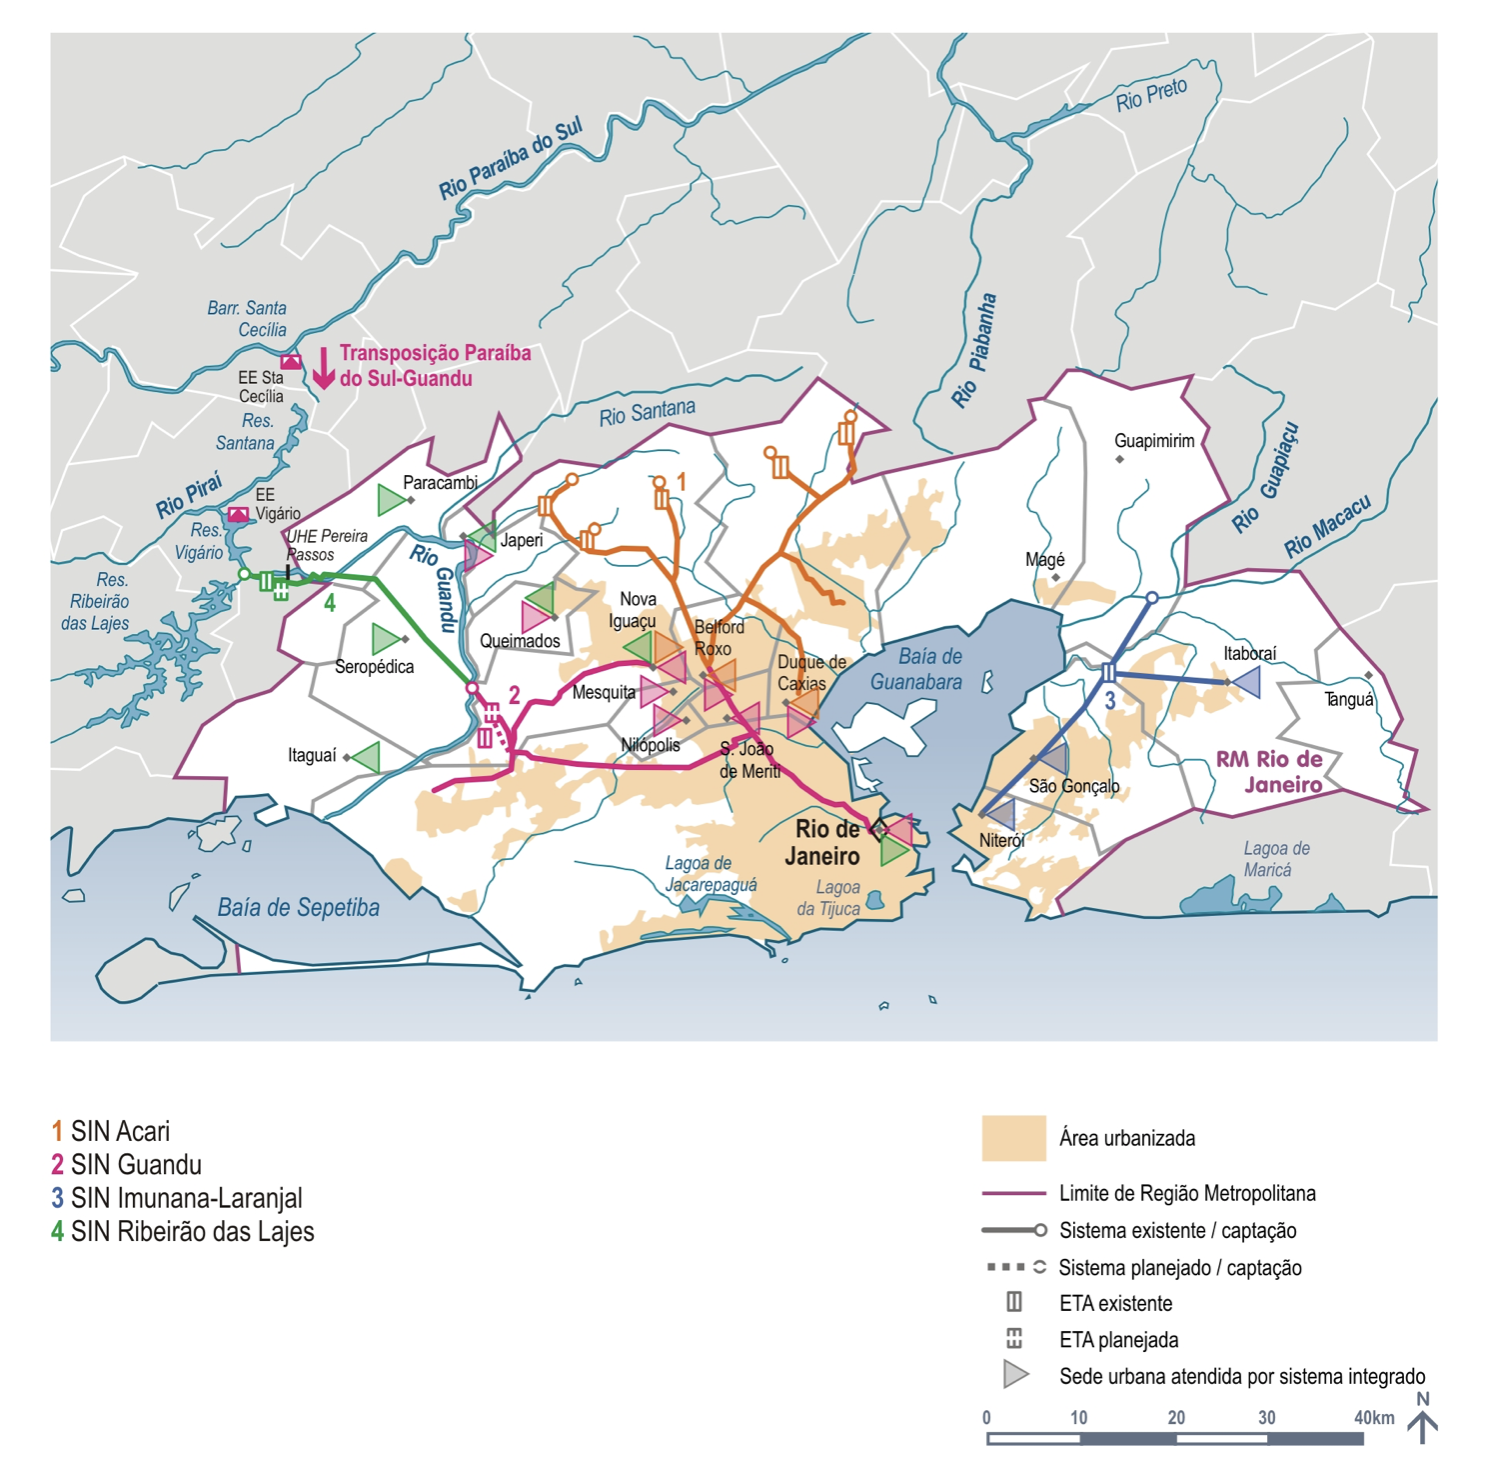
\includegraphics[width=0.8\linewidth]{imagem/abastece} 

}

\caption{Abastecimento de água da RM do Rio de Janeiro.}\label{fig:unnamed-chunk-2}
\end{figure}
\centerline{Fonte: www.ana.gov.br.}

Em 23 de janeiro, a CEDAE divulgou nota informando que iniciaria processo licitatório no valor de 90 milhões de reais para a realização de obras visando a ``proteção da tomada de água da estação de tratamento de água (ETA) Guandu''. Anunciou, ainda, que irá investir 700 milhões de reais até 2022 nesta mesma estação de tratamento.

No dia 29 de janeiro, a companhia anunciou o início da utilização de argila ionicamente modificada com o objetivo de ``impedir a proliferação excessiva de algas que possam interferir no tratamento da água'' utilizada no ETA Guandu.

No dia 03 de fevereiro \citep{Ana-ebc2}, foi detectada a presença de detergente nas águas do rio Guandu e a CEDAE decidiu fechar as comportas da estação de tratamento de água de Guandú, interrompendo a produção por treze horas. Ao retomar a produção, a concessionária informou que poderia levar até 3 dias para o fornecimento se normalizar.

No dia 04 de junho, a impressa divulga laudo elaborado pela Universidade Federal do Rio de Janeiro (UFRJ). Neste laudo é apresentado o resultado de análises realizadas nas água do rio Guandu. Ainda, é informado que foram encontradas grandes quantidades de esgoto domestico e industrial, bem como grandes quantidades de bactérias de origem fecal, um forte indício de contaminação por esgoto \citep{chicor}.

No mesmo dia, a CEDAE voltou a tratar do tema em uma nota de esclarecimento na qual informa que a geosmina, assim como o 2-Metil-Isoborneol, causam alterações de gosto e odor da água, mas que não são prejudiciais para a saúde. Informa também que a companhia está monitorando a quantidade destas duas substâncias e destaca que desde fevereiro não ocorrem alterações decorrentes destas duas substâncias.

A CEDAE é uma empresa do setor de saneamento, do tipo sociedade de economia mista, que presta serviço para o estado do Rio de Janeiro. No período de 2007 a 2010, a empresa passou por uma reestruturação visando a abertura de capital \citep{novacedae}. Entretanto, atualmente, 99,99\% da empresa pertence ao governo do estado do Rio de Janeiro.

Conforme \citet{crisecedae}, apesar da reestruturação da gestão, o problema de contaminação com geosmina ocorrido em janeiro de 2020, é visto como resultado de um baixo investimento em saneamento básico por parte da empresa, além de investimentos pouco efetivos. A baixa cobertura dos serviços de coleta e tratamento de esgoto resultam em poluição dos afluentes do rio Guandu, levando, em última análise, com que a ETA Guandu precise tratar água com qualidade próxima a de esgoto. As autoras do estudo efetuaram uma comparação entre o desempenho da CEDAE e outras três empresas do mesmo setor (COPASA-MG, SABESP-SP e SANEPAR-PR). Destas empresas, apenas a CEDAE apresentou uma tragetória decrescente quanto ao percentual de coleta e tratamento de esgoto no período de 2010 a 2018. O valor investido por habitante também foi o menor dentre as quatro empresas.

Em estudo realizado pela Firjan, foi avaliada a necessidade de investimentos para realizar a expansão dos serviços de saneamento básico no estado do Rio de Janeiro. Essa expansão visa alcançar a meta de ``100\% dos domicílios atendidos com abastecimento de água e 96\% com coleta e tratamento de esgoto, até 2033''. Segundo o estudo, seriam necessários R\$ 20,1 bilhões, até 2033, para alcançar a meta estipulada de cobertura de 89 municípios.

\hypertarget{intro}{%
\chapter{Metodologia}\label{intro}}

\hypertarget{descriuxe7uxe3o-do-local-do-estudo}{%
\section{Descrição do local do estudo}\label{descriuxe7uxe3o-do-local-do-estudo}}

O estudo foi conduzido no estado do Rio de Janeiro. Estado cuja capital possui o mesmo nome. Conforme dados do Instituto Brasileiro de Geografia e Estatística (IBGE), o estado do Rio de Janeiro é composto por 92 municípios e possui uma população de 17.366.189 habitantes, sendo que apenas na capital residem 6.747.815 pessoas (2019, IBGE). A densidade demográfica do estado é de 365 habitantes por quilômetro quadrado, sendo que, na área metropolitana esse valor sobe para 1226 habitantes e na capital esse valor é de 5265 habitantes por quilômetro quadrado. Cerca de 97\% da população do estado vive em área urbana e 52\% da população é do sexo feminino.Quanto a estrutura etária, 6\% da população está na faixa de menor que 5 anos e 8,9\% da população tem mais de 65 anos. A média de moradores por unidade domiciliar é de três habitantes. O indice de desenvolvimento humano (IDH) do estado está em 0,761 e o rendimento mensal domiciliar per capita é de R\$ 1.882,00 (em 2019, segundo IBGE).

Para avaliar o impacto causado na capital (município do Rio de Janeiro), foi selecionado o município de Niterói como grupo controle. Embora este município também faça parte da região metropolitana, não houve relatos deste problema, pois é abastecido por outra estação de tratamento, a de Imunana-Laranjal que utiliza as águas dos rios Macacu e Guapiaçu.

\begin{figure}

{\centering 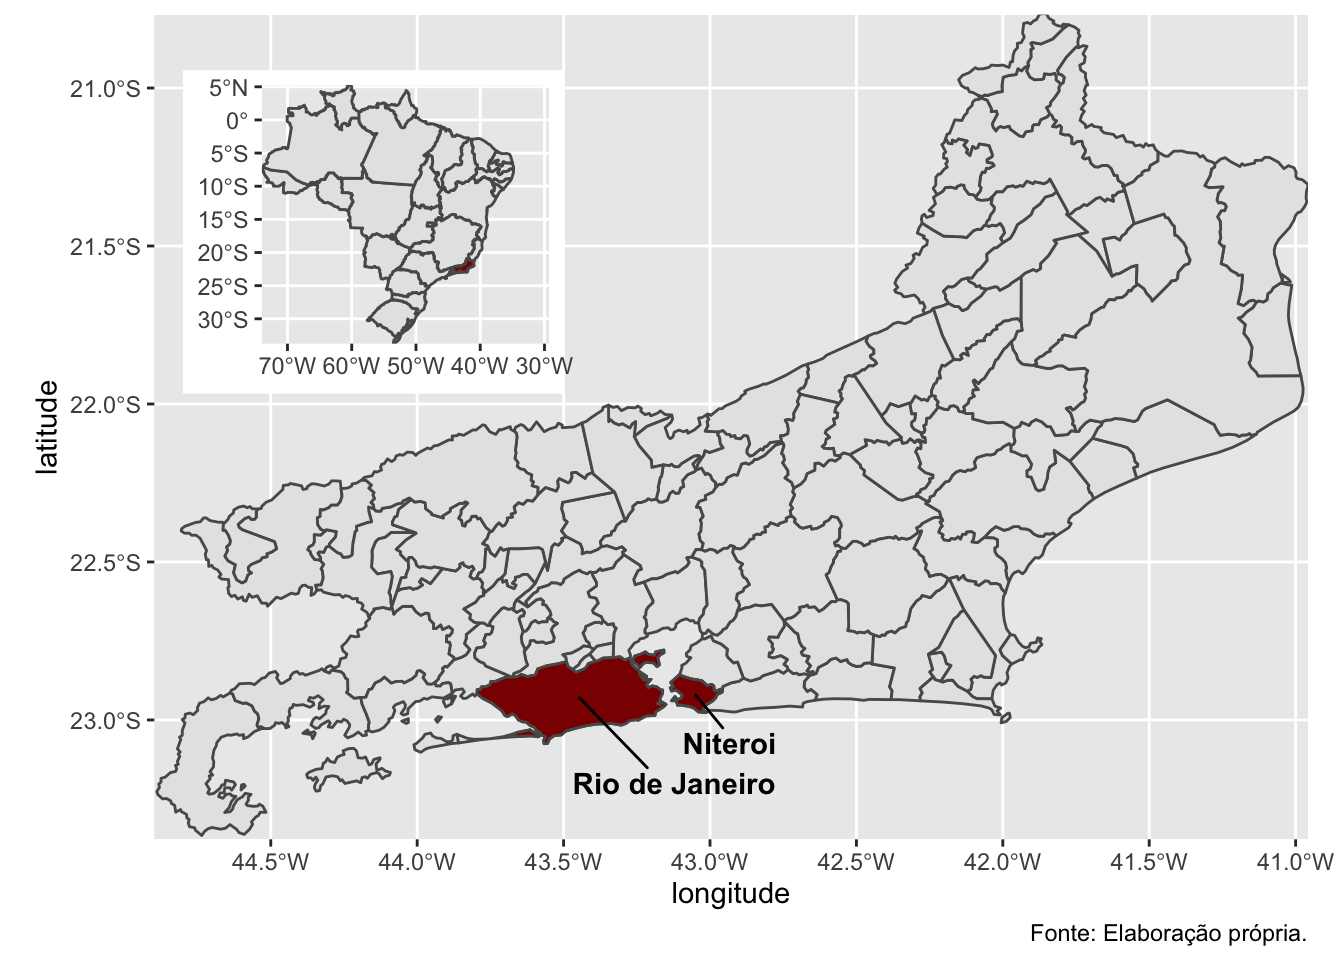
\includegraphics{dissertacao-demo_files/figure-latex/unnamed-chunk-6-1} 

}

\caption{Localização dos municípios estudados.}\label{fig:unnamed-chunk-6}
\end{figure}

\hypertarget{levantamento-e-anuxe1lise-dos-dados}{%
\section{Levantamento e análise dos dados}\label{levantamento-e-anuxe1lise-dos-dados}}

\hypertarget{venda-de-uxe1gua-mineral}{%
\subsection{Venda de água mineral}\label{venda-de-uxe1gua-mineral}}

Foram utilizados dados obtidos na Secretaria de Fazenda do Estado do Rio de Janeiro decorrentes da venda de agua mineral no varejo. Os dados extraidos foram: dia do ano, endereço do ponto de venda (bairro,rua, número, município e CEP), decrição do produto e GTIN de cada produto vendido em cada ponto de venda naquele dia, preços praticados no dia de cada produto em cada ponto de venda e a quantidade vendida no dia para cada produto, em cada ponto de venda, naquele dia. Os dados utilizados são dos municípios do Rio de Janeiro e do município de Niterói, no período entre 01 de dezembro de 2019 e 25 de março de 2020.

Na fase de limpeza dos dados, os mesmos foram filtrados por GTIN , sigla de ``\emph{global trade item number}'' (também conhecido por código EAN, referente a ``\emph{european article number}''). O GTIN é um número utilizado abaixo dos códigos de barras e serve para que o fabricante possa identificar de forma única o seu produto.

Foram selecionados os 30 GTINs que representavam os 30 produtos mais vendidos no período analisado. Estes produtos representavam 75\% do total vendido. Desta forma foram excluidos 25\% dos dados entre os quais se encontra a maior parte dos dados de baixa qualidade (onde há grande quantidade de erros), que demandariam grande esforço de limpeza, agregando pouca informação adicional. Dos 30 GTINs, foram analisadas suas descrições e extraida a informação do volume em ml das garrafas de água mineral.

A partir do CEP dos pontos de venda, realizou-se o cruzamento com os CEPs de cada área de ponderação (AP) para descobrir de qual AP determinado ponto de venda pertencia, o que permitiu a realização de um cruzamento com os dados do cadastro nacional de endereços para fins estatísticos (CNEFE) do IBGE. Em alguns casos, o CEP estava em duas APs. Nesse caso, os dados de endereço dos pontos de venda foram utilizados para fazer o georreferenciamento, ou seja, levantar quais são a latitude e longitude dos pontos de venda para saber a qual área de ponderação pertencia.

A partir deste ponto os GTINs foram removidos e os pontos de vendas tiveram seus dados de endereço e geolocalização retirados, ficando somente a informação da área de ponderação a que pertence determinado dado. Com isso, a análise dos dados passou a ocorrer de forma agragada \footnote[1]{Conforme Portaria RFB n 2344/11, artigo 2, parágrafo 1 "não estão protegidas pelo sigilo fiscal as informações agregadas, que não identifiquem o sujeito passivo."}, visando respeitar o sigilo fiscal.

\hypertarget{uxe1reas-de-ponderauxe7uxe3o-e-dados-socioeconuxf4micos}{%
\subsection{Áreas de ponderação e dados socioeconômicos}\label{uxe1reas-de-ponderauxe7uxe3o-e-dados-socioeconuxf4micos}}

\begin{figure}

{\centering 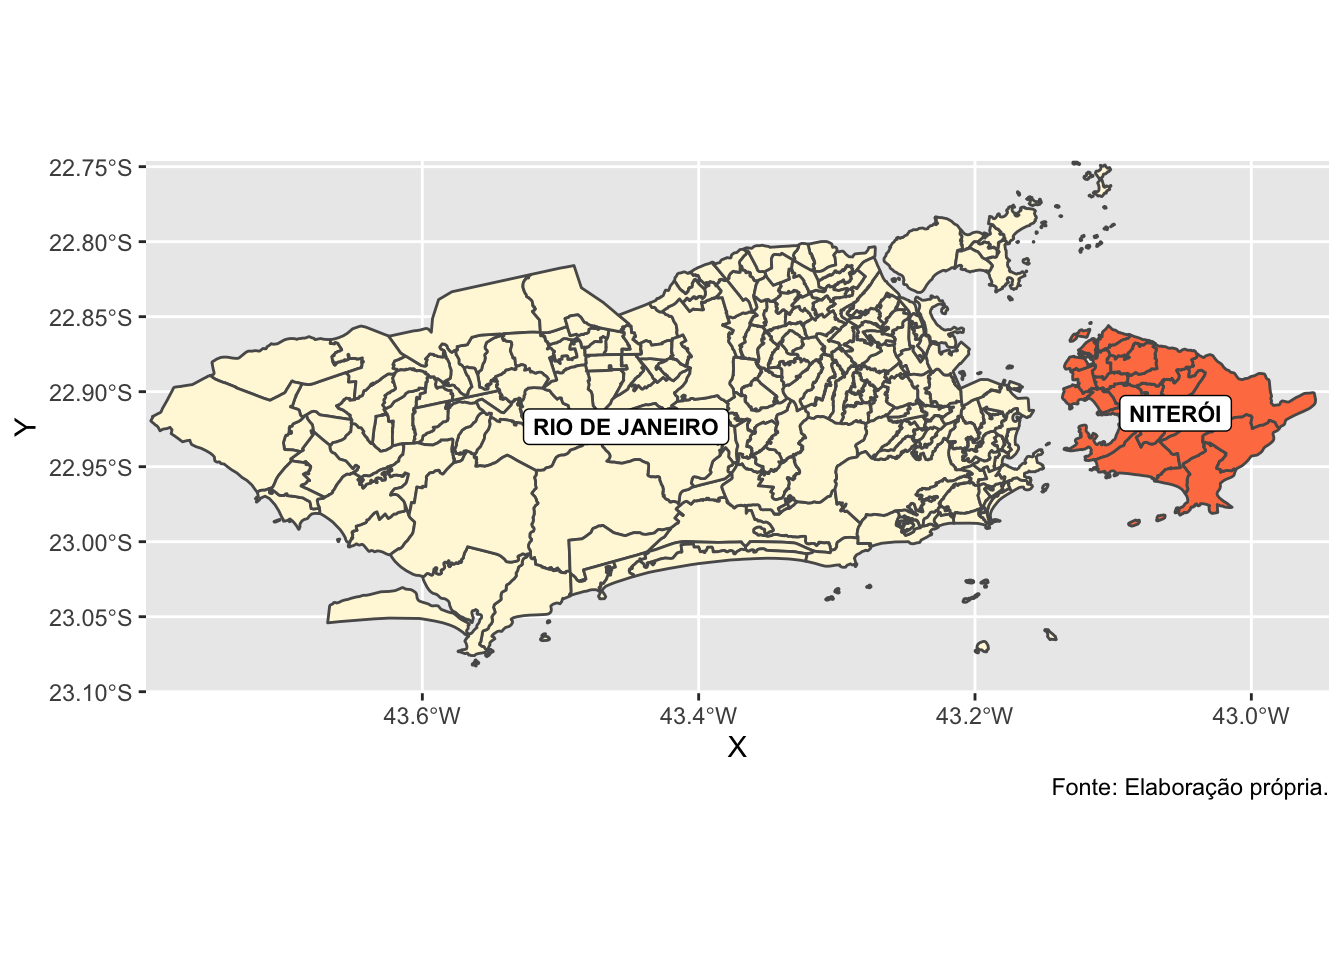
\includegraphics[width=0.9\linewidth]{dissertacao-demo_files/figure-latex/apond-1} 

}

\caption{Divisão em áreas de ponderação.}\label{fig:apond}
\end{figure}

Conforme já mencionado, os dados foram agregados por área de ponderação . As áreas de ponderação (figura \ref{fig:apond}) são áreas definidas pelo IBGE para fins de levantamentos estatísticos. Desde 1960 o IBGE realiza, a cada dez anos, censos demográficos no Brasil com metodologia de amostragem para levantamento de dados sociodemográficos, entre outros. As áreas de ponderação (AP) são a menor unidade territorial para a qual o IBGE divulga seus microdados, tendo em vista a necessidade de proteger a confidencialidade das informações.

O tamanho de uma área de ponderação é variável e está relacionado ao desenho amostral utilizado pelo IBGE.O menor tamanho de uma AP é de 400 domicílios particulares ocupados na amostra. Estas amostras são selecionadas de forma independente por amostragem aleatória simples sem reposição. Para o domicílio selecionado, são levantadas informações de todos os moradores.

Os dados do censo precisam de tratamento adequado pois existem as questões de probabilidades desiguais de seleção, além de observações com pesos desiguais, entre outros. Questões que foram levadas em consideração no presente trabalho. Para esta etapa foi utilizado o pacote \emph{Survey} \citep{psurvey} do R.

Os mapas das APs são disponibilizados no \emph{site} do IBGE. com base nesses mapas foram realizados os georreferenciamentos dos pontos de vendas. Além disso, foram levantados os dados de renda per capita, idade, escolaridade e sexo para as APs estudadas, a partir dos microdados do censo de 2010 do IBGE.

\hypertarget{temperatura}{%
\subsection{Temperatura}\label{temperatura}}

Tendo em vista que altas temperaturas podem influenciar no consumo de água mineral, foram levantados os dados de temperatura para cada dia estudado. Os dados de temperatura foram obtidos de estação meteorológica situada no aeroporto Santos Dumond. Este dado foi obtido através do \emph{site} do \emph{National Oceanic and Atmospheric Administration}, o qual reune, de forma padronizada, dados climáticos de mais de 29 mil pontos ao redor do mundo.

A escolha deste aeroporto ocorreu pois o mesmo se situa em região limítrofe entre os dois municípios estudados (Rio de Janeiro e Niterói). Foram obtidos dados de temperatura de hora em hora. Em seguida foi utilizada a temperatura mais alta do dia. Nesta etapa foi utilizado o pacote \emph{stationaRy} \citep{stationaRy} do R.

\hypertarget{anuxe1lise-dos-dados}{%
\subsection{Análise dos dados}\label{anuxe1lise-dos-dados}}

Para análise dos dados foi utilizado o pacote estatístico R \citep{R-base}. A análise foi realizada com a utilização do pacote plm \citep{plm}.

Para formatação do trabalho foi utilizado como referencia o trabalho de \citet{xie2015}.

\hypertarget{analise-das-variuxe1veis}{%
\chapter{Analise das Variáveis}\label{analise-das-variuxe1veis}}

\begin{figure}

{\centering 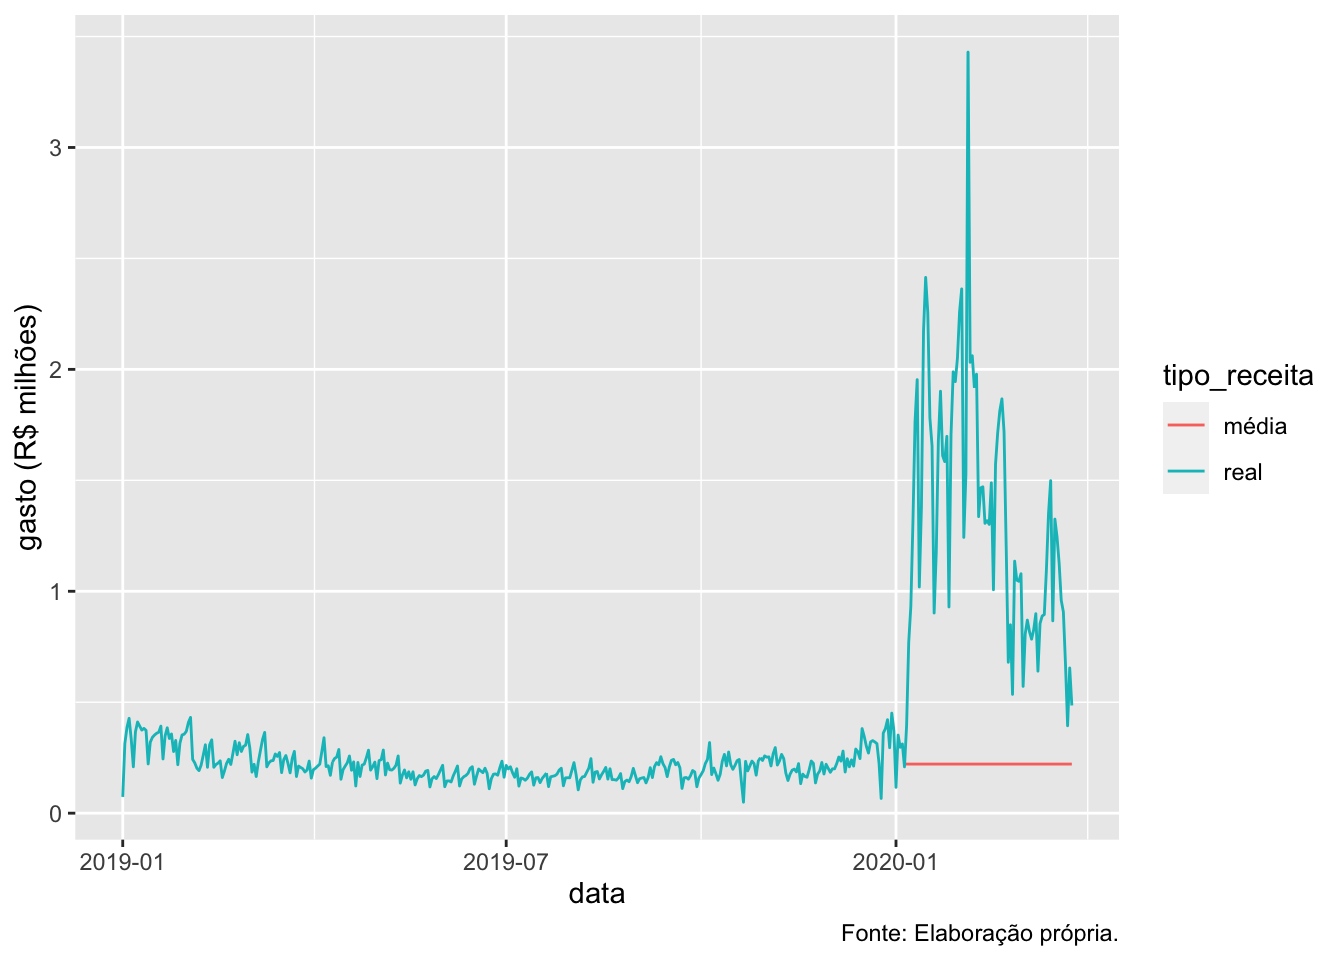
\includegraphics{dissertacao-demo_files/figure-latex/grafico1-1} 

}

\caption{Gasto diário com água mineral}\label{fig:grafico1}
\end{figure}

Conforme gráfico \ref{fig:grafico1}, podemos observar o comportamento dos gastos com água mineral durante o ano de 2019 e no primeiro trimestre de 2020. Durante o ano de 2019 é possível observar um padrão na receita decorrente da venda de água mineral em um patamar abaixo de R\$ 500 mil. Já no ano de 2020 o comportamento sofre uma brusca alteração. E esta alteração pode ser melhor observada no gráfico \ref{fig:grafico2}.

\begin{figure}

{\centering 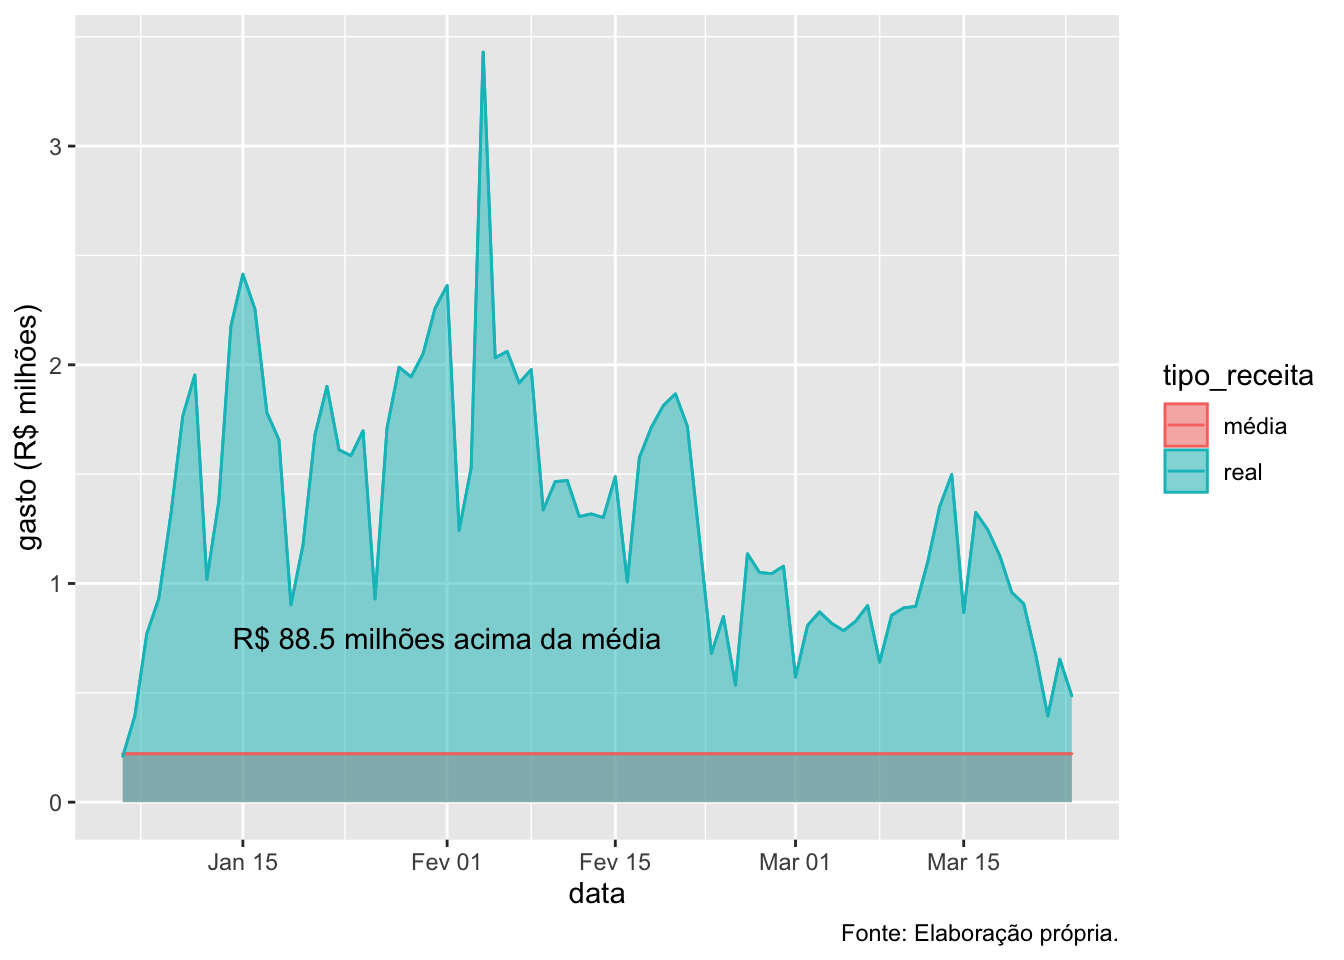
\includegraphics{dissertacao-demo_files/figure-latex/grafico2-1} 

}

\caption{gasto diário com água mineral durante a crise hídrica.}\label{fig:grafico2}
\end{figure}

Este gráfico demonstra a variação nos gastos com água mineral no período do evento. A linha em vermelho representa uma projeção do gasto com água mineral a partir dos dados de 2019 (com os dados de 2019 utilizou-se um modelo arima para prever 2020). A linha em vermelho representa o valor esperado com base nos dados de 2019. A linha em azul representa o valor realmente observado.

Aplicando a diferença entre as áreas sob as duas curvas é possível inferir o impacto do evento no município.

\[\int_{jan}^{mar} receita_{observada} - \int_{jan}^{mar} receita_{estimada}\]

A diferença calculada foi de aproximadamente R\$ 88.5 milhões acima da média, conforme está representado no gráfico \ref{fig:grafico2}.

\begin{figure}

{\centering 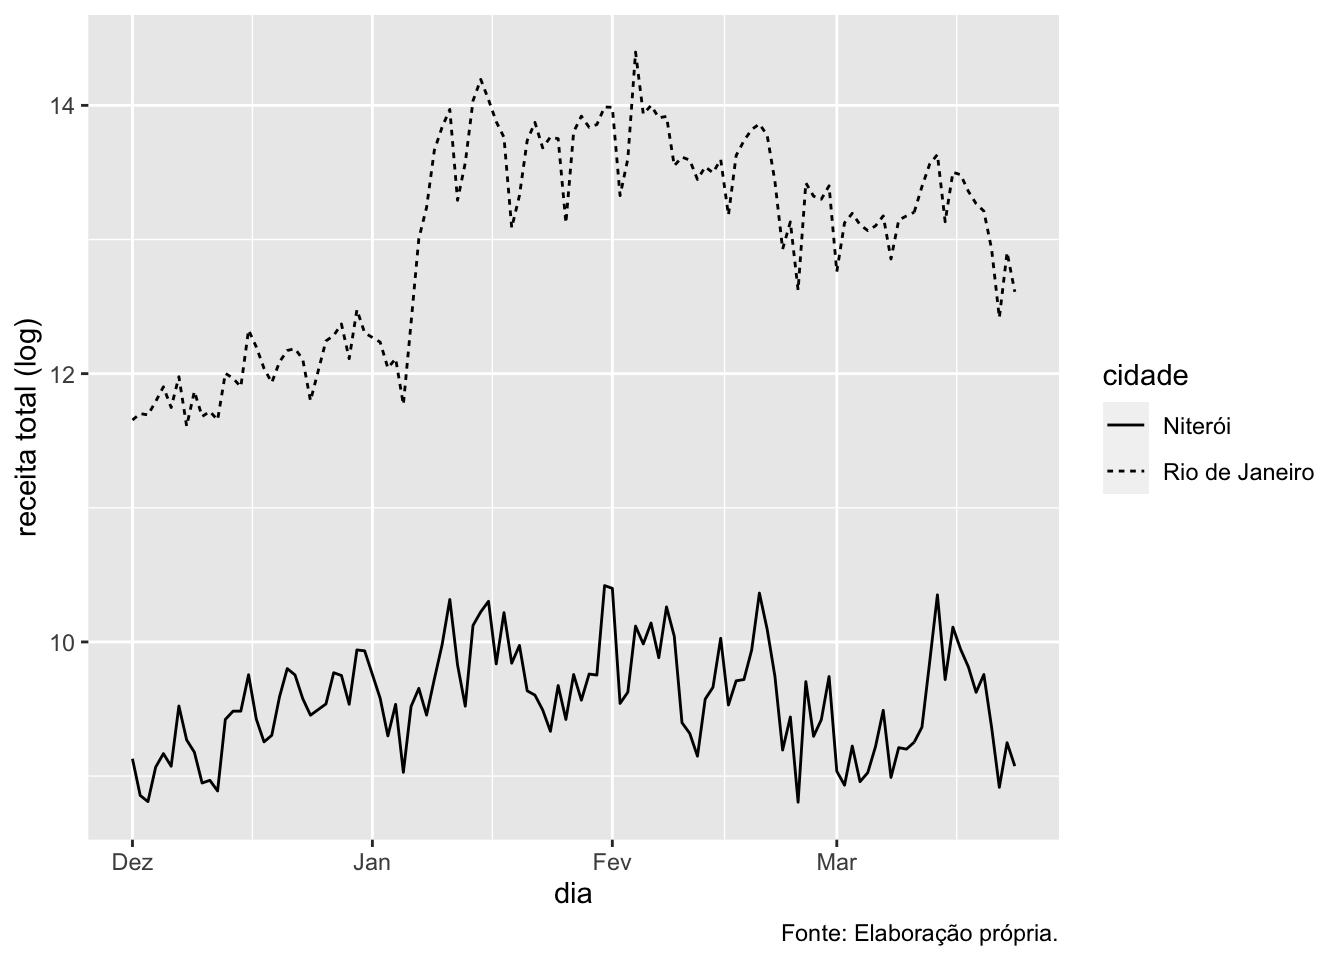
\includegraphics{dissertacao-demo_files/figure-latex/grafico3-1} 

}

\caption{receita total em log.}\label{fig:grafico3}
\end{figure}

O gráfico \ref{fig:grafico3} apresenta a receita total (preço x quantidade) de cada dia no município do Rio de Janeiro (linha tracejada) e no município de Niterói (linha cheia) das vendas de garrafas de água. Os valores são apresentados após transformação logarítmica para melhor visualização. Apesar da forte alteração observada no município do Rio de Janeiro, no município do Niterói não é observada alteração no padrão da receita.

\begin{figure}

{\centering 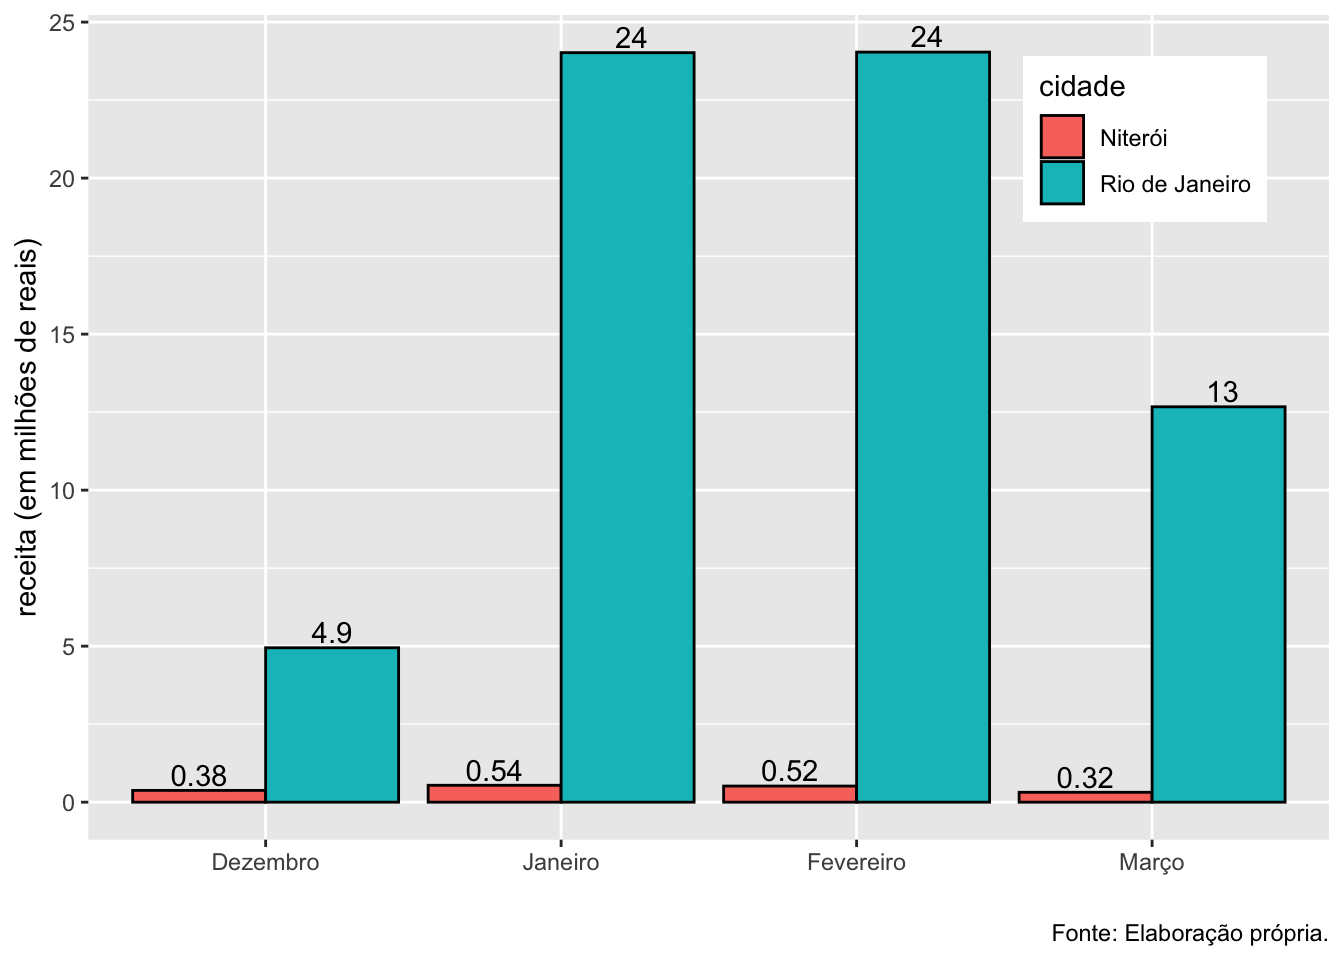
\includegraphics{dissertacao-demo_files/figure-latex/grafico4-1} 

}

\caption{receita por mês no período de dez/19 a mar/20}\label{fig:grafico4}
\end{figure}

Adotando uma outra abordagem, os dados foram agrupados por município e por mês. Desta forma é possível observar (figura \ref{fig:grafico4}) o impacto mensal do evento no município do Rio de Janeiro. Enquanto em dezembro de 2019 a receita total ficou em R\$ 5 milhões, em janeiro, ou seja quando ocorreu o evento, a receita passou para R\$ 24 milhões, representando um aumento de 380\%.

\hypertarget{preuxe7o-e-quantidade-consumida-de-uxe1gua-mineral}{%
\section{Preço e quantidade consumida de água mineral}\label{preuxe7o-e-quantidade-consumida-de-uxe1gua-mineral}}

\begin{figure}

{\centering 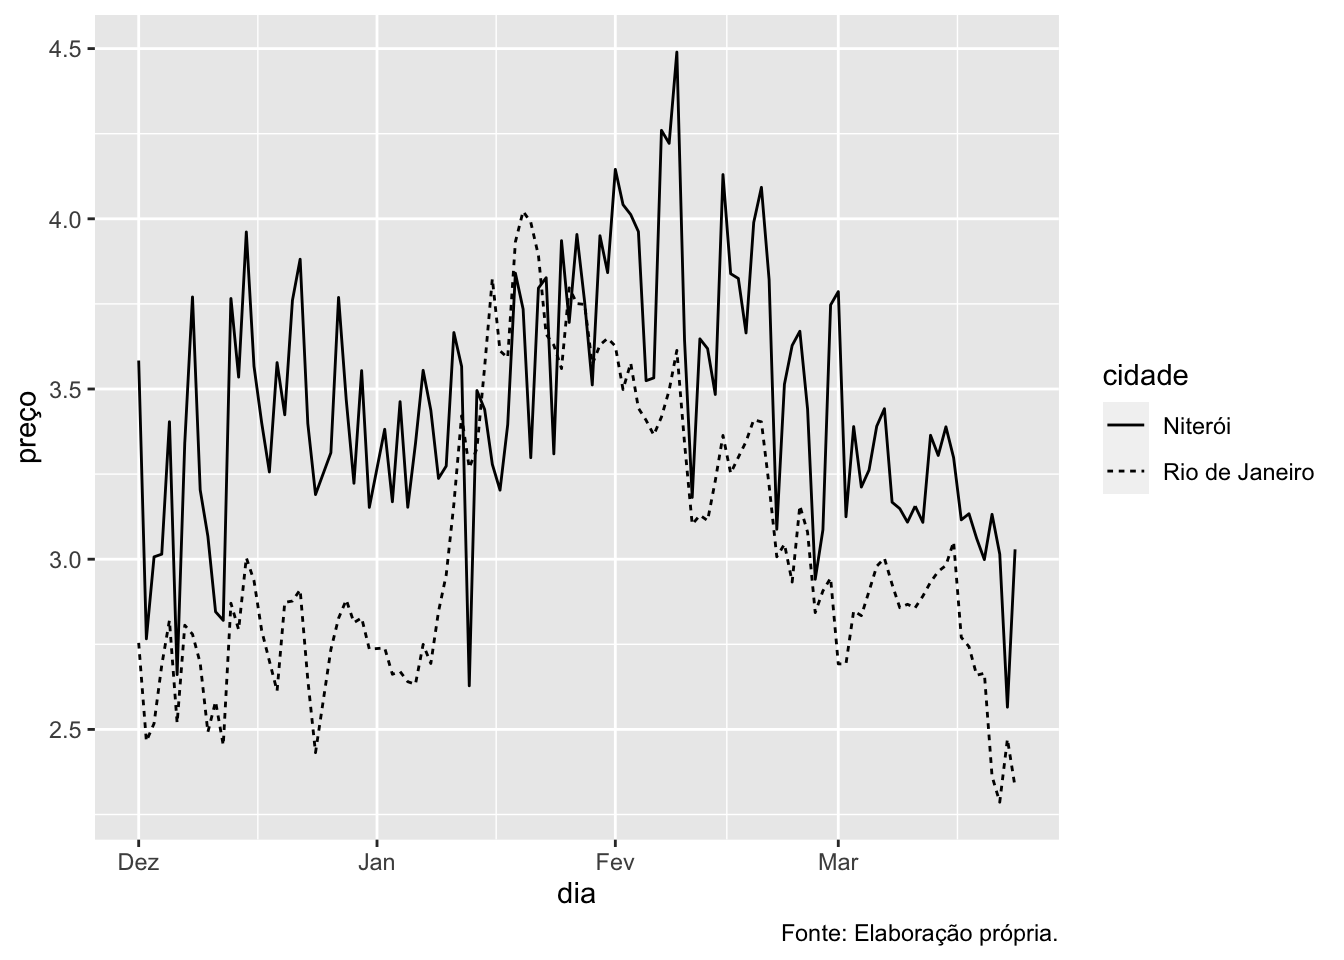
\includegraphics{dissertacao-demo_files/figure-latex/preco-1} 

}

\caption{acompanhamento da média de preços}\label{fig:preco}
\end{figure}

O gráfico \ref{fig:preco} apresenta a média de preço ao longo do tempo no município do Rio de Janeiro (linha tracejada) e no município de Niterói (linha cheia) do litro de água mineral. É possível observal que em Niterói, dada sua proximidade com o local do evento, ainda que não tenha sido afetada de forma direta, seus preços foram afetados. Entretanto, o impacto nos preços foi menor em Niterói quando comparado ao município do Rio de Janeiro.

\begin{figure}

{\centering 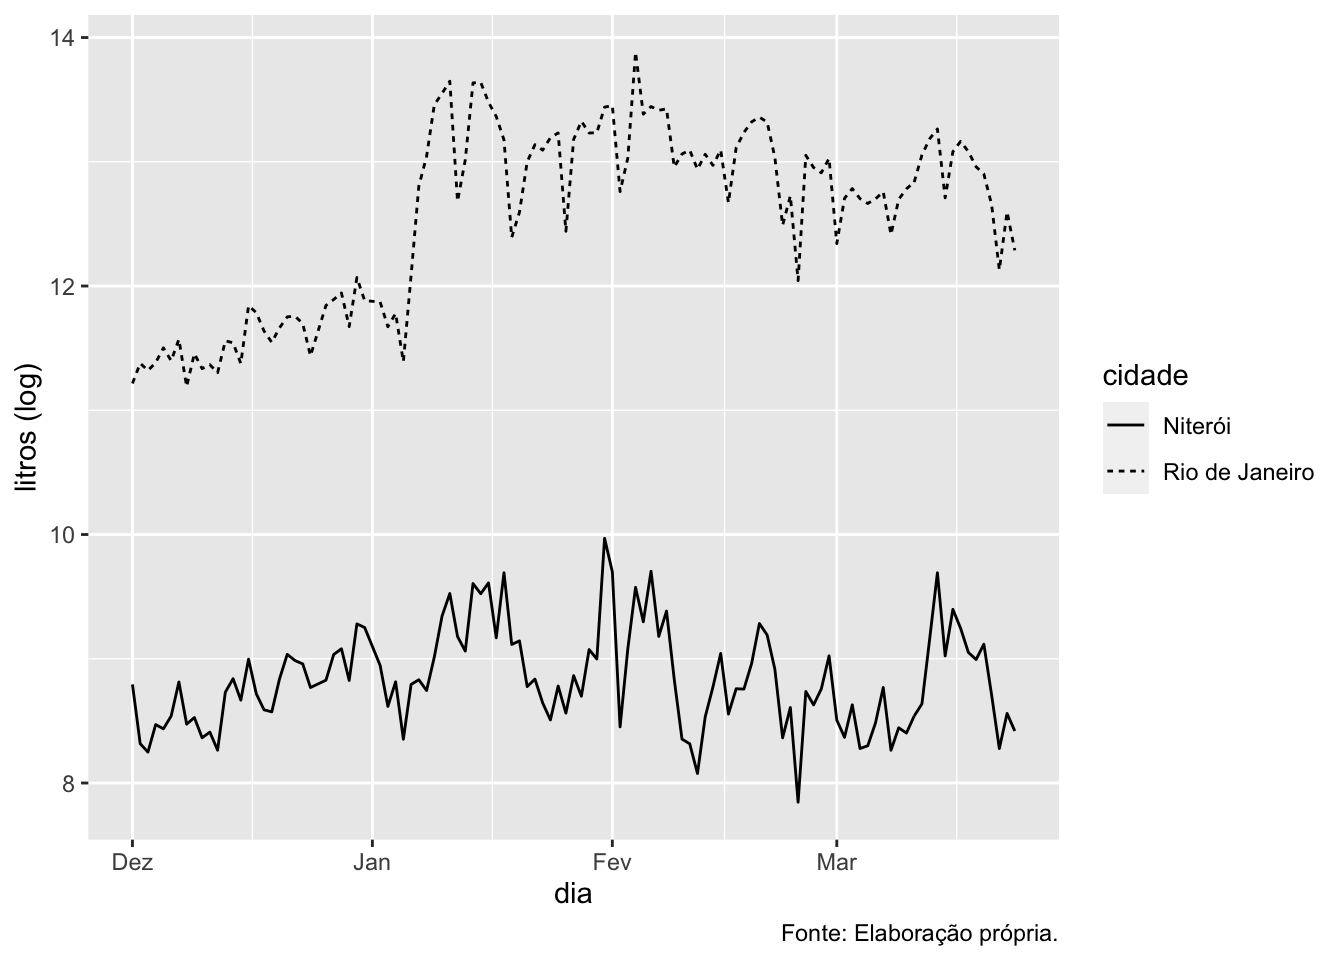
\includegraphics{dissertacao-demo_files/figure-latex/quantidade-1} 

}

\caption{consumo (em log) em litros.}\label{fig:quantidade}
\end{figure}

O gráfico \ref{fig:quantidade} apresenta a quantidade vendida ao longo do tempo no município do Rio de Janeiro (linha tracejada) e no município de Niterói (linha cheia) em litros (valores em log para melhor visualização). No município do Rio de Janeiro, antes do evento, as vendas raramente alcançavam 162 mil litros (\(\exp{12}\) = 162.754,8). Após o evento a quantidade vendida passa a girar entorno de 442 mil litros/dia (\(\exp{13}\) = 442.413,4). Em niterói não houve variação na quantidade consumida, ficando próximo de 8 mil litros/dia (\(\exp{9}\) = 8.103,1).

\hypertarget{dados-do-censo-2010-e-distribuiuxe7uxe3o-espacial}{%
\section{Dados do censo 2010 e distribuição espacial}\label{dados-do-censo-2010-e-distribuiuxe7uxe3o-espacial}}

\hypertarget{renda}{%
\subsection{Renda}\label{renda}}

Os dados foram agregados por área de ponderação (AP). A variável renda apresentou uma forte correlação espacial. É possível perceber na figura \ref{fig:mapa1} uma concentração das regiões de alta renda per capita. No mapa, as áreas em cinza são regiões que foram descartadas por falta de dados de consumo de água mineral.

\begin{figure}

{\centering 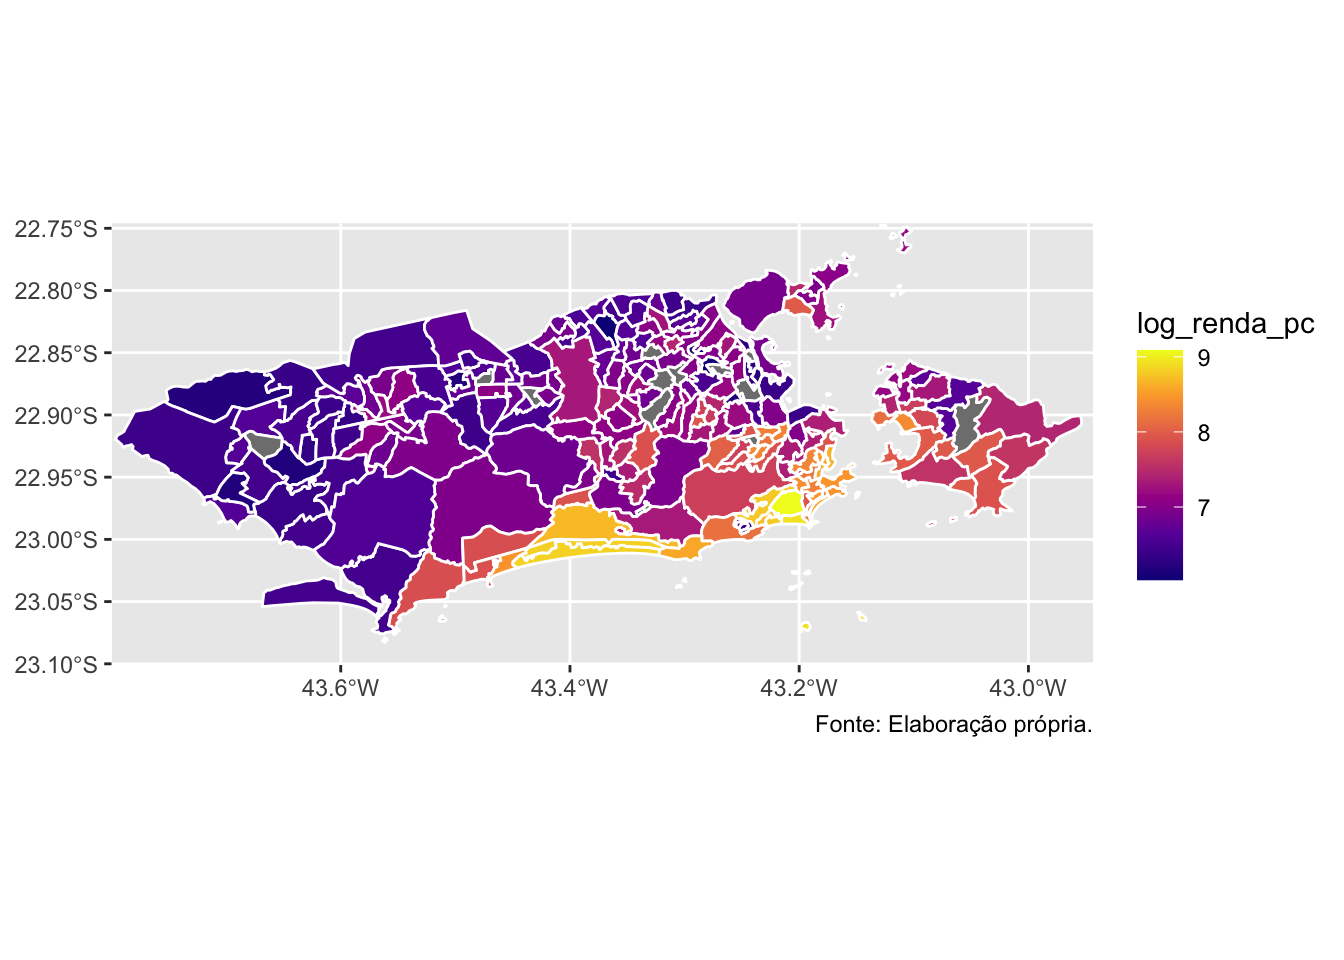
\includegraphics{dissertacao-demo_files/figure-latex/mapa1-1} 

}

\caption{Renda per capita (log)}\label{fig:mapa1}
\end{figure}

\newpage

\hypertarget{escolaridade}{%
\subsection{Escolaridade}\label{escolaridade}}

A variável escolaridade foi avaliada pela proporção de pessoas com nível superior completo em cada AP. Pela figura \ref{fig:mapa2} podemos perceber que esta variável apresenta distribuição semelhante a da renda per capita.

\begin{figure}

{\centering 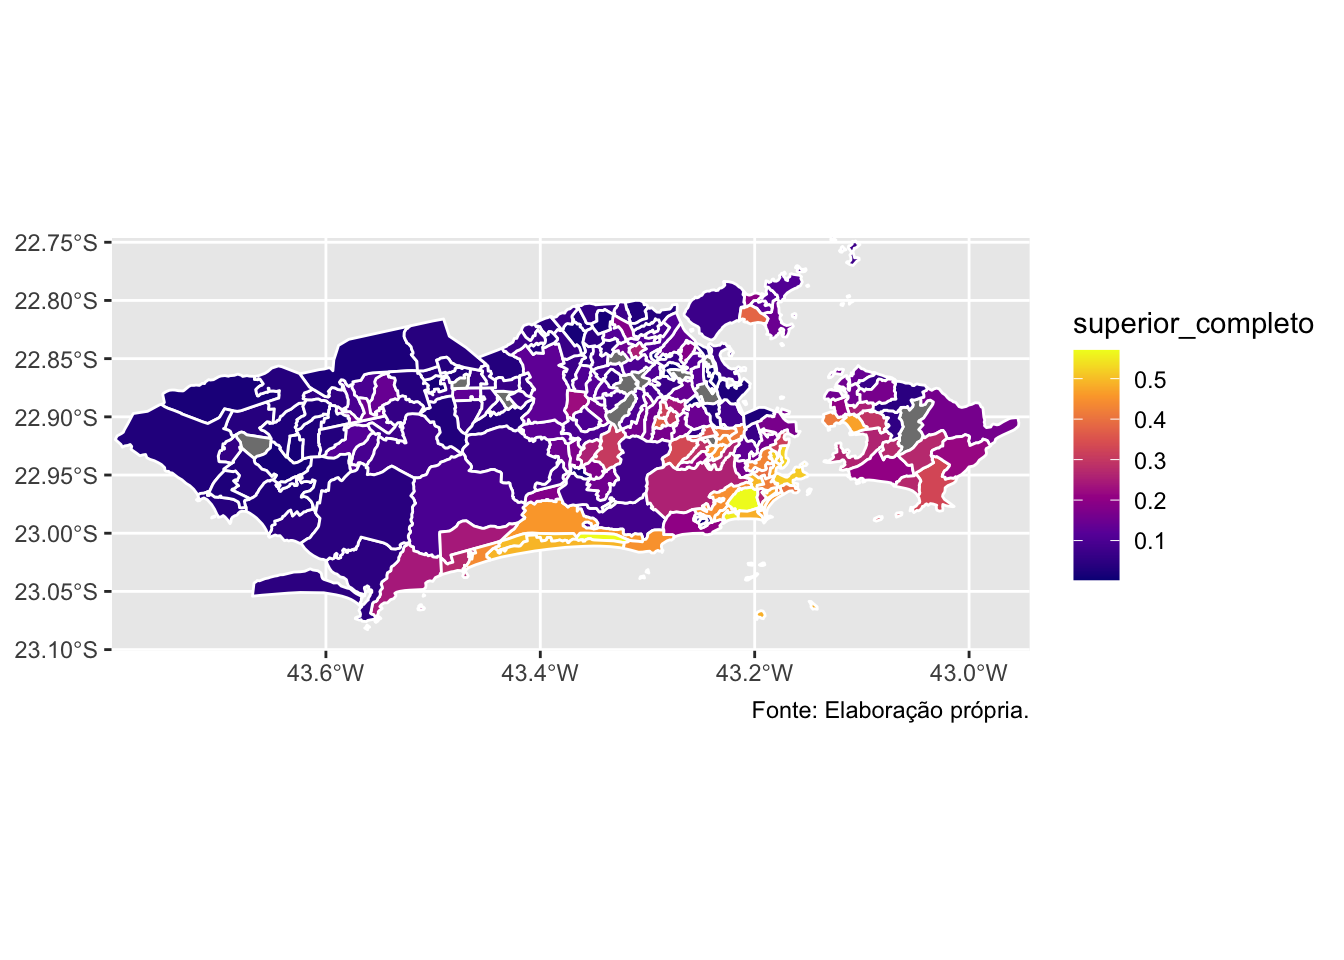
\includegraphics{dissertacao-demo_files/figure-latex/mapa2-1} 

}

\caption{proporção de pessoas com nivel superior completo (0/1).}\label{fig:mapa2}
\end{figure}

\newpage

\hypertarget{sexo}{%
\subsection{Sexo}\label{sexo}}

A variável sexo foi avaliada pela proporção de mulheres em cada AP. A figura \ref{fig:mapa3} apresenta a distribuição espacial desta variável. Pode-se perceber um possível outlier nesta variável.

\begin{figure}

{\centering 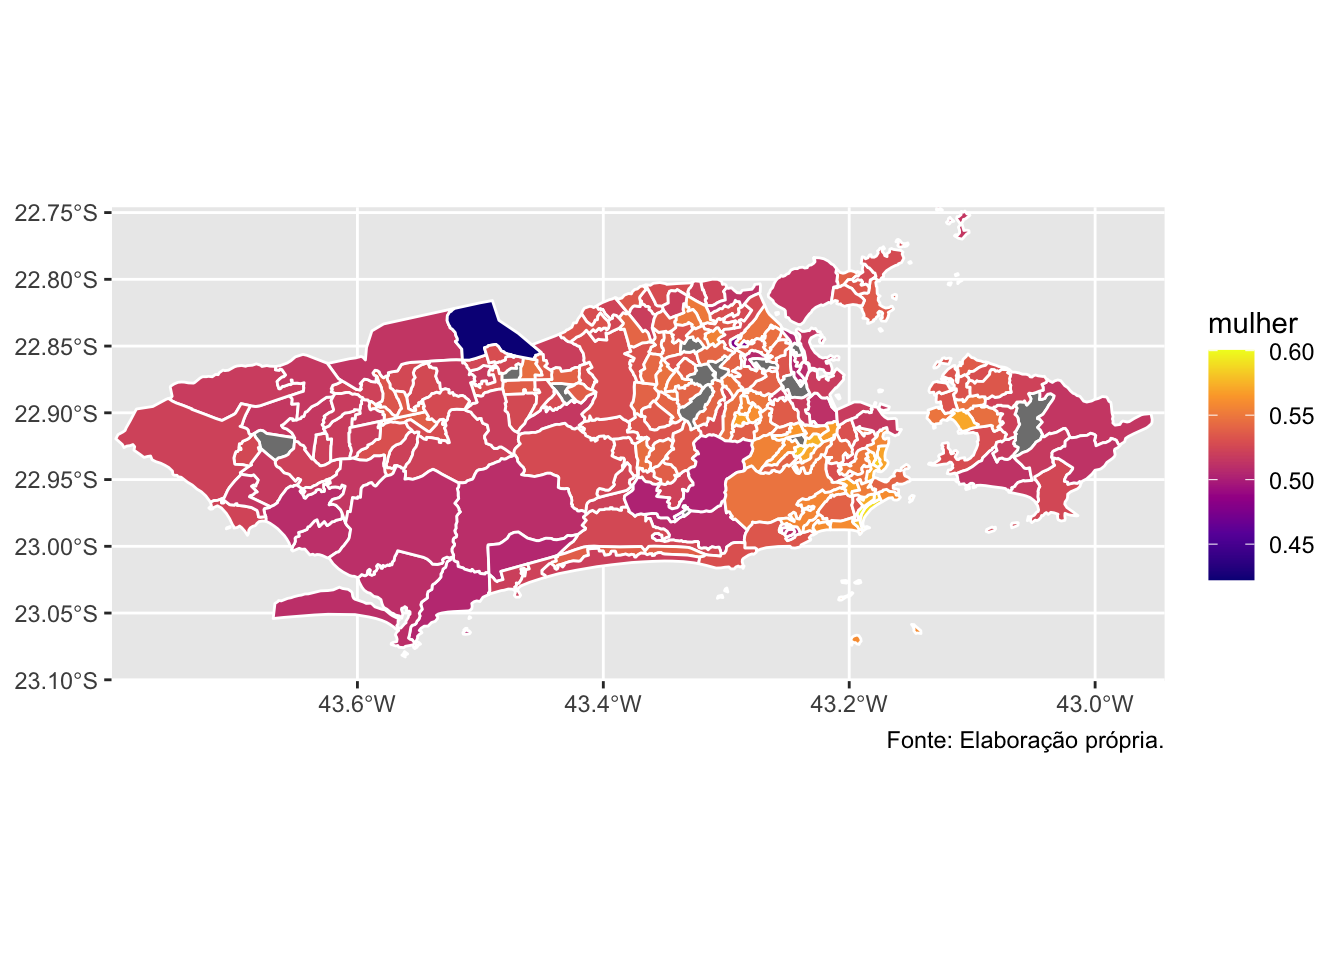
\includegraphics{dissertacao-demo_files/figure-latex/mapa3-1} 

}

\caption{proporção de mulheres (0/1).}\label{fig:mapa3}
\end{figure}

\newpage

\hypertarget{idade}{%
\subsection{Idade}\label{idade}}

Para avaliar o impacto da variável idade foi detacada a proporção de crianças menores de três anos em cada AP. Tal abordagem é decorrência da literatura que aponta a existência de correlação entre crianças e a demanda por água. Além disso, como já destacado, o público infantil é o que apresenta maior risco decorrente de água de má qualidade. A Figura \ref{fig:mapa4} apresenta a distribuição deste parâmetro.

\begin{figure}

{\centering 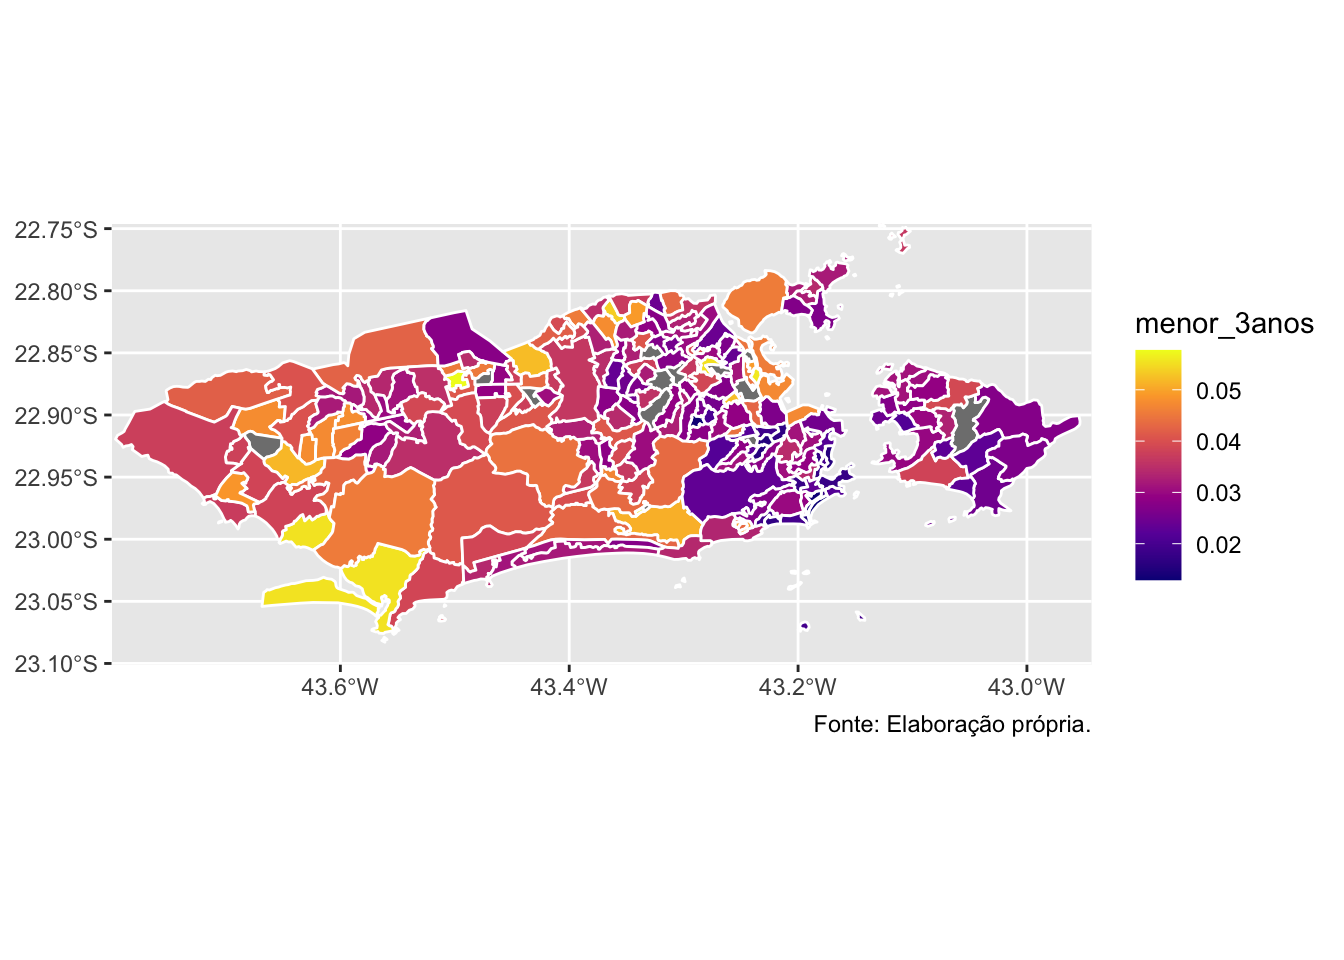
\includegraphics{dissertacao-demo_files/figure-latex/mapa4-1} 

}

\caption{proporção de crianças menores de 3 anos (0/1).}\label{fig:mapa4}
\end{figure}

\hypertarget{receita-total}{%
\section{Receita total}\label{receita-total}}

Em um primeiro momento, para avaliar a disposição a pagar foi selecionado o mês de fevereiro de 2020. Os dados foram agrupados por areas de ponderação. Conforme Figura \ref{fig:wtprenda} abaixo, o WTP foi medido com um percentual da renda domiciliar. Neste estágio, a renda domiciliar média foi multiplicada por um fator visando sua atualização. Este fator foi obtido pela razão entre as rendas de 2010 (censo 2010, IBGE) e de 2019 (PNAD 2019, IBGE) do município do Rio de Janeiro.

\begin{figure}

{\centering 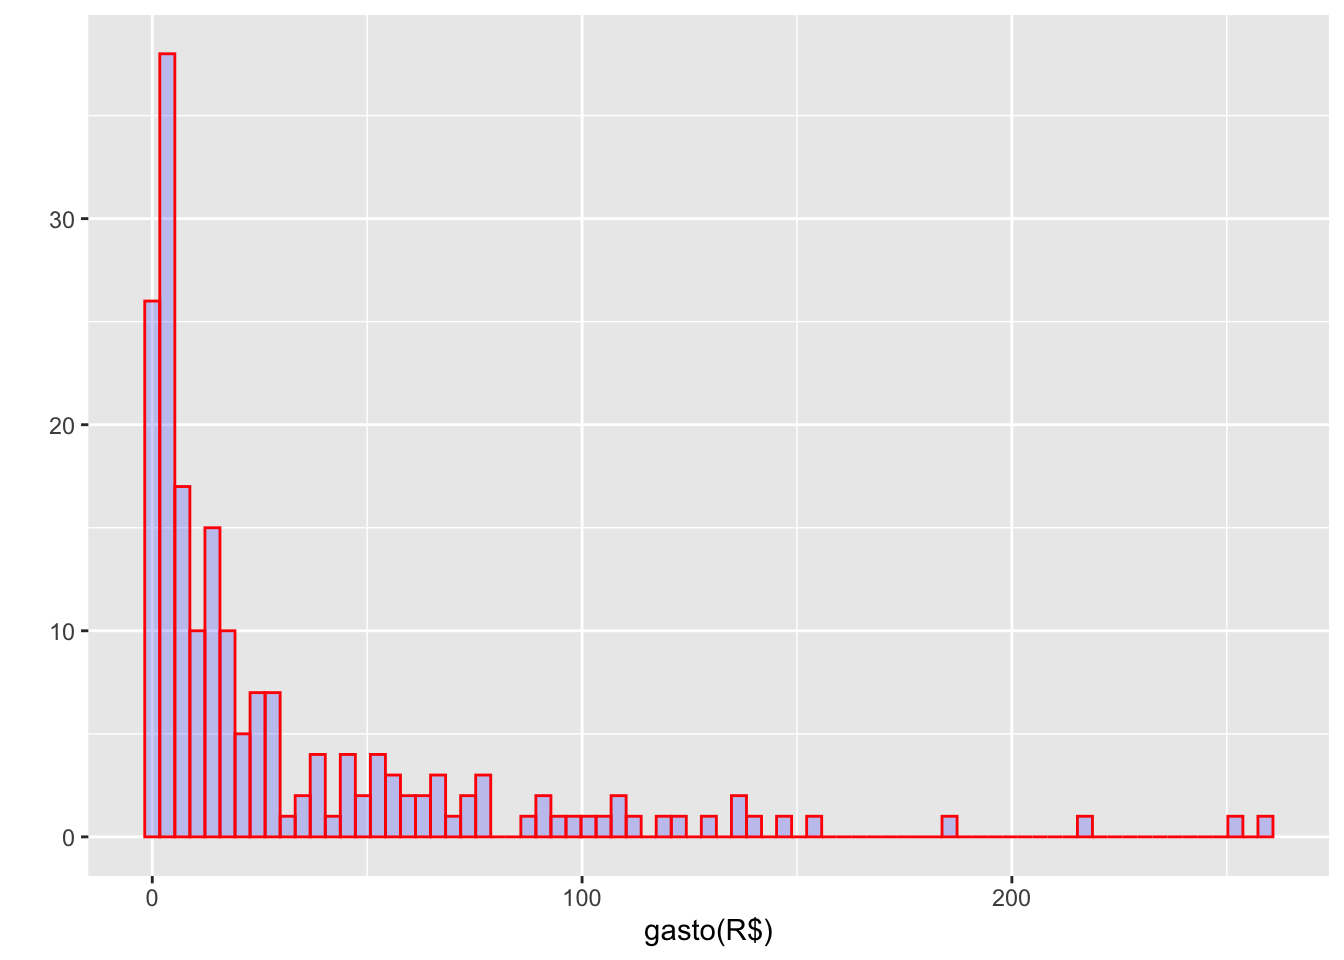
\includegraphics{dissertacao-demo_files/figure-latex/wtprenda-1} 

}

\caption{gasto em percentual da renda domiciliar}\label{fig:wtprenda}
\end{figure}

Conforme figura \ref{fig:wtprenda}, foi observado um gasto médio de R\$ 31,72 ( U\$ 7.89 pela cotação de 02/01/2020) por domicílio. Estudo de \citet{wtpmalawi} observou um WTP variando de U\$ 0,95 a U\$ 111,38 com uma média de U\$ 10,73.

Outro estudo realizado no Espírito Santo, Brasil, \citep{wtpespiritosanto} os autores encontraram um valor de WTP de U\$ 3,0 por mês. Neste estudo foram mensurados os gastos realizados para obter água para consumo em uma população com acesso a água encanada, mas com serviço intermitente. Foram avaliados gastos para ferver ou filtrar água e com a compra de água engarrafada. Apenas 4\% da população estudada utilizava a água engarrafada e 70\% utilizava filtros.

\begin{table}

\caption{\label{tab:regreceita}Resultado da regressão múltipla sobre a receita total das vendas}
\centering
\begin{tabular}[t]{l|r|r|r|r}
\hline
term & estimate & std.error & statistic & p.value\\
\hline
(Intercept) & 134693.04 & 1432843.33 & 0.09 & 0.93\\
\hline
mulher & -70226.20 & 2572861.25 & -0.03 & 0.98\\
\hline
superior\_completo & -124159.23 & 886917.96 & -0.14 & 0.89\\
\hline
rendaDomiciliar & 70.03 & 32.24 & 2.17 & 0.03\\
\hline
menor\_3anos & -838715.17 & 5656766.87 & -0.15 & 0.88\\
\hline
\end{tabular}
\end{table}

Na tabela \ref{tab:regreceita}, foi realizada uma regressão para estimar quais variáveis impactam na receita total de vendas de água mineral. Apenas a renda domiciliar mostrou relação estatisticamente significante com a receita.

\begin{figure}

{\centering 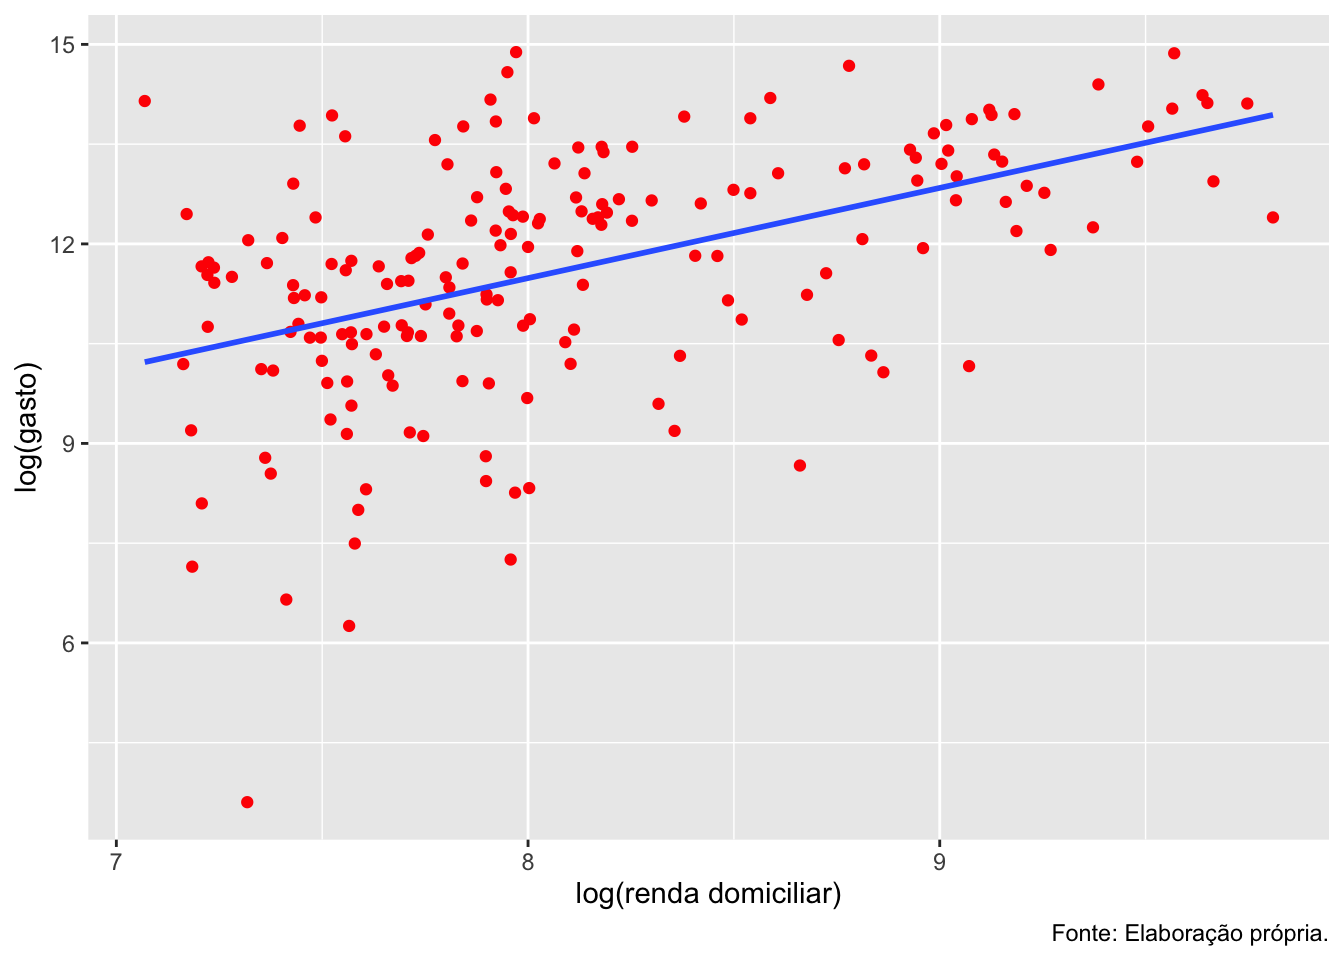
\includegraphics{dissertacao-demo_files/figure-latex/unnamed-chunk-29-1} 

}

\caption{Gráfico da renda domiciliar e gastos com água mineral.}\label{fig:unnamed-chunk-29}
\end{figure}

Acima, gráfico das variáveis renda domiciliar e receita total.

\begin{figure}

{\centering 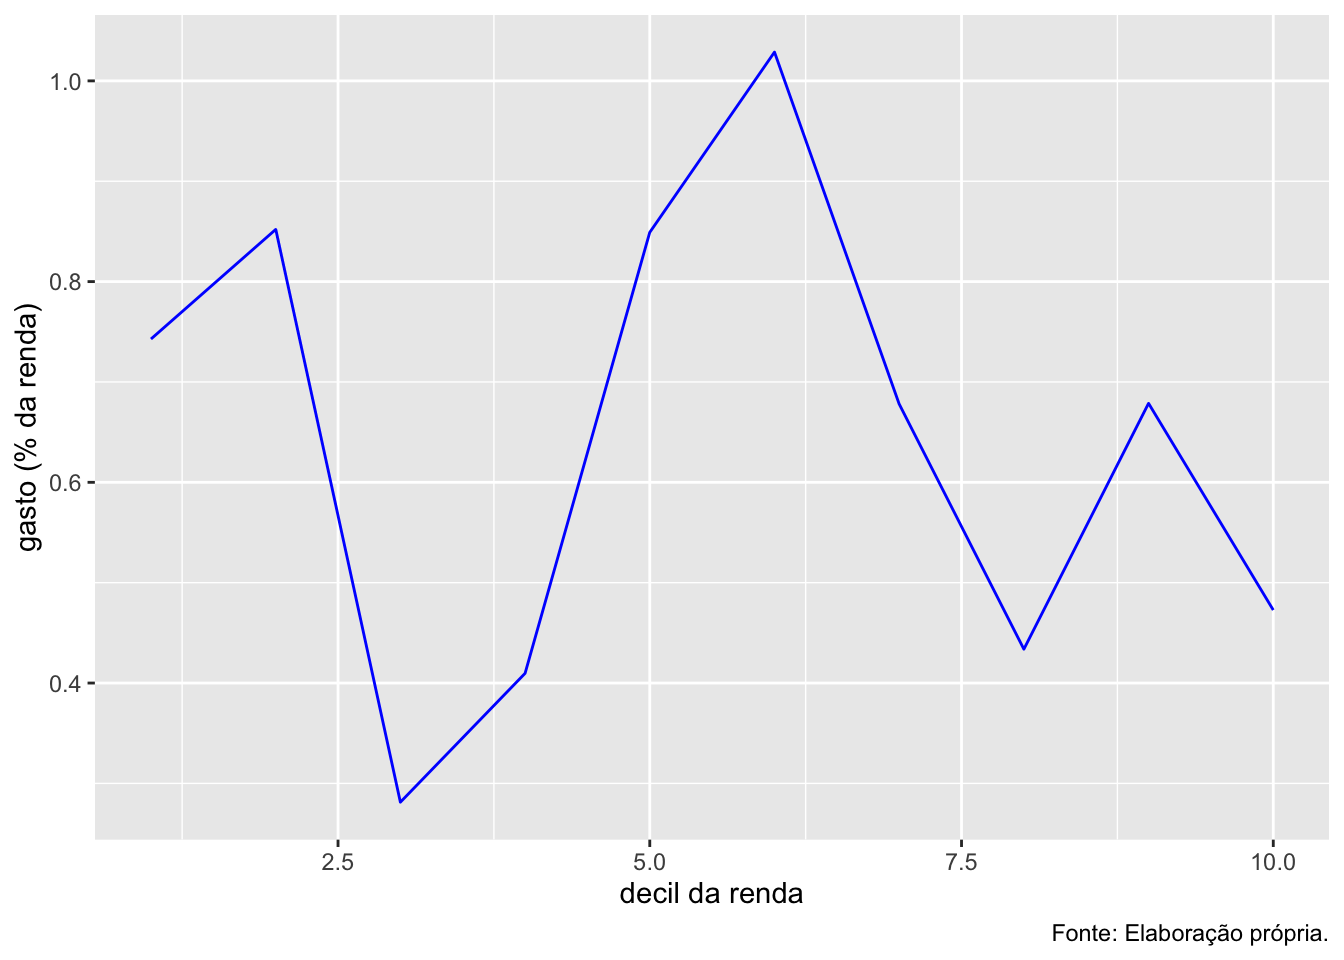
\includegraphics{dissertacao-demo_files/figure-latex/unnamed-chunk-30-1} 

}

\caption{Relação entre gasto e decis de renda.}\label{fig:unnamed-chunk-30}
\end{figure}

No gráfico acima, foi avaliado como se comporta o gasto (expresso em \% da renda domiciliar) em relação aos decis de renda (os dados foram agrupados em decis de renda). O quantil de renda grupo 1 seria os 10\% mais pobres e o grupo 10 seriam os 10\% mais ricos. Com base no gráfico, não é possível observar uma tendencia linear. Entretanto, observa-se que o impacto é maior nos grupos 5 e 6. Nos extremos o impacto é menor, o que pode ser explicado pelo baixo impacto no orçamento do grupo mais rico de comprar água mineral e no grupo mais pobre talvez garrafas de água mineral não seja a primeira opção de substituição. Outras opções seriam utilizar filtros ou ferver a água. Além disso, o presente estudo não alcança o consumo de galões de água de 20 litros, o que é bastante utilizado em regiões onde o serviço de água encanada é deficiente.

\hypertarget{inferindo-o-impacto}{%
\chapter{Inferindo o impacto}\label{inferindo-o-impacto}}

Para estimar a demanda de água mineral, em um primeiro momento, é preciso lidar com o problema da causalidade simultânea, a qual é decorrente do fato de que a quantidade afeta o preço ao mesmo tempo em que o preço afeta a quantidade. Desta forma, o preço passa a ser uma variável endógena, situação que viola hipotese básica do modelo dos mínimos quadrados (OLS). A literatura apresenta alternativas para lidar com esse problema, sendo utilizado no presente trabalho a técnica das variáveis instrumentais, ou regressão em dois estágios (2SLS).

Tal técnica se utiliza de uma terceira variável (instrumento) a qual precisa atender a duas condições para que seja valida \citep{stockwatson} que são a relevância do instrumento e exogeneidade do instrumento. Ou seja, dado um instrumento \(Z\) e uma variável explicativa endógena \(X\), a relevância do instrumento implica em \(corr(Z,X) \not= 0\) e a exogeneidade do instrumento implica em \(corr(Z,u)=0\), sendo \(u\) o resíduo.

Desta forma, para estimar a elasticidade preço da demanda, dado por:

\[ Q = \beta_0 + \beta_1P + u_i \]

O primeiro estágio utiliza \(Z\) para estimar a parte de \(P\) não influenciada por \(Q\):

\[ \hat{P} = \pi_0 + \pi_1Z_i + v_i\]

No segundo estágio utiliza-se o \(\hat{P}\), que é o preço estimado sem a influência de \(Q\), para estimar o impacto de \(P\) em \(Q\).

\[ Q = \beta_0 + \beta_1\hat{P} + u_i  \]

Desta maneira, o coeficiente \(\beta_1\) não será viesado.

O teste para avaliar a força da variável instrumental foi realizada com o teste F para o primeiro estágio. O teste assume a hipótese nula de que a variável instrumental é fraca.

O teste de Wu-Hausman avalia a consistência dos estimadores. Apresenta a hipótese nula de que a endogeneidade não está presente na regressão, não sendo necessário recorrer a IV (variáveis instrumentais).

Após lidar com a questão da causalidade simultânea, as regressões foram realizadas com os dados em painel\citep{colonescu}, onde os mesmos foram agragados por semana e por AP. A análise em painel ocorre quando há dados de diversos indivíduos ao longo do tempo. Nesta etapa duas metodologias foram utilizadas: modelo de dados agregados e modelo de efeitos fixos.

Na primeira etapa foi realizada uma análise com os dados agregados.

\begin{equation} 
  y_{it} = \beta_{1} + \beta_{2}x_{2it} + ... + \beta_{k}x_{kit} + \xi_{it}
  \label{eq:pooled}
\end{equation}

Conforme equação \eqref{eq:pooled}, onde i representa cada unidade de observação e t representa a variável tempo. Em seguida, os dados foram análisados utilizando o modelo de efeitos fixos, coforme equação \eqref{eq:fixed}.

\begin{equation} 
  y_{it} = \beta_{1i} + \beta_{2}x_{2it} + ... + \beta_{k}x_{kit} + \xi_{it}
  \label{eq:fixed}
\end{equation}

Como é possível observar, a diferença da equação \eqref{eq:fixed} em relação a equação \eqref{eq:pooled} está no intercepto, posto que este modelo leva em consideração diferenças entre indivíduos. Este modelo é utilizado para contornar o viés da variável omitida. Com isso, esse modelo assume a existência de interceptos distintos para cada unidade observacional \(i\).

\hypertarget{na-quantidade-via-demanda-de-uxe1gua-mineral}{%
\section{Na quantidade via demanda de água mineral}\label{na-quantidade-via-demanda-de-uxe1gua-mineral}}

A seguir, são apresentados os resultados dos modelos utilizados.

\begin{table}

\caption{\label{tab:demagreg}modelo agregado}
\centering
\begin{tabular}[t]{l|r|r|r|r}
\hline
term & estimate & std.error & statistic & p.value\\
\hline
(Intercept) & -20.570 & 2.834 & -7.259 & 0.000\\
\hline
aguaRuimTRUE & 1.303 & 0.116 & 11.239 & 0.000\\
\hline
log\_media\_preco & -1.606 & 0.455 & -3.532 & 0.000\\
\hline
log(refri1) & 1.188 & 0.481 & 2.468 & 0.014\\
\hline
log\_renda\_pc & 1.158 & 0.087 & 13.312 & 0.000\\
\hline
log(temp\_media) & 5.626 & 0.842 & 6.680 & 0.000\\
\hline
\end{tabular}
\end{table}

\begin{table}

\caption{\label{tab:demfe}modelo de efeitos fixos}
\centering
\begin{tabular}[t]{l|r|r|r|r}
\hline
term & estimate & std.error & statistic & p.value\\
\hline
aguaRuimTRUE & -3.411 & 3.510 & -0.972 & 0.331\\
\hline
log\_media\_preco & 29.577 & 23.345 & 1.267 & 0.205\\
\hline
log(refri1) & -5.669 & 4.765 & -1.190 & 0.234\\
\hline
log(temp\_media) & -18.537 & 20.066 & -0.924 & 0.356\\
\hline
\end{tabular}
\end{table}

\begin{table}

\caption{\label{tab:demre}modelo de efeitos aleatórios}
\centering
\begin{tabular}[t]{l|r|r|r|r}
\hline
term & estimate & std.error & statistic & p.value\\
\hline
(Intercept) & -20.638 & 2.815 & -7.332 & 0.000\\
\hline
aguaRuimTRUE & 1.299 & 0.115 & 11.266 & 0.000\\
\hline
log\_media\_preco & -1.612 & 0.454 & -3.552 & 0.000\\
\hline
log(refri1) & 1.193 & 0.480 & 2.484 & 0.013\\
\hline
log\_renda\_pc & 1.168 & 0.086 & 13.501 & 0.000\\
\hline
log(temp\_media) & 5.628 & 0.837 & 6.726 & 0.000\\
\hline
\end{tabular}
\end{table}

As tabelas \ref{tab:demagreg}, \ref{tab:demfe} e \ref{tab:demre} apresentam os resultados dos modelos agregado, de efeitos fixos e de efeitos aleatórios. No modelo agregado observa-se um coeficiente de 1,314 para a variável água ruim. Todas as variáveis apresentaram significância estatística, exceto as faixas etárias. No modelo de efeitos aleatórios, a variável água ruim passa a ter um coeficiente de 1,311.

\begin{table}

\caption{\label{tab:testinstrument}teste do instrumento da função demanda}
\centering
\begin{tabular}[t]{l|r|r}
\hline
  & statistic & p-value\\
\hline
Weak instruments & 189.09 & 0\\
\hline
Wu-Hausman & 15.90 & 0\\
\hline
\end{tabular}
\end{table}

Conforme tabela \ref{tab:testinstrument} a hipótese nula de que a variável instrumental é fraca foi rejeitada, demonstrando a necessidade da utilização de IV. Os testes permitem concluir a existência de endogeneidade, assim como, que a variável utilizada como instrumento é adequada.

Para avaliar a demanda de água mineral foi utilizada como variável instrumental o preço de bebidas adicionadas de açúcar ou de outros edulcorantes ou aromatizadas e outras bebidas não alcoólicas (NCM: 2202.10.00).

\begin{table}

\caption{\label{tab:testf}Teste para efeitos fixos na função demanda}
\centering
\begin{tabular}[t]{r|r|r|r|l|l}
\hline
df1 & df2 & statistic & p.value & method & alternative\\
\hline
176 & 2285 & -11.5867 & 1 & F test for individual effects & significant effects\\
\hline
\end{tabular}
\end{table}

Foi utilizado o teste-F para comparar o modelo agregado e o modelo de efeitos fixos. A tabela \ref{tab:testf} mostra que a hipótese nula (em que não há efeitos fixos) é rejeitada. Portanto, o modelo de efeitos fixos é mais adequado do que o modelo agregado.

\begin{table}

\caption{\label{tab:randomt2}Teste de efeitos aleatórios para a equação da demanda}
\centering
\begin{tabular}[t]{r|r|l|l}
\hline
statistic & p.value & method & alternative\\
\hline
72.25034 & 0 & Lagrange Multiplier Test -  (Honda) for unbalanced panels & significant effects\\
\hline
\end{tabular}
\end{table}

Em seguida foi testada a presença de efeitos aleatórios. Conforme tabela \ref{tab:randomt2}, a hipótese nula de que a variância é zero para cada região foi rejeitada. Ou seja, a heterogeneidade nas regiões é significante.

Tendo em vista que neste modelo, o evento água ruim foi representado por uma dummy e que o modelo de efeitos aleatórios é o mais adequado, a regressão log-nível apresentou um coeficiente de 1,311. Desta forma, pode-se dizer que o evento, quando ocorre, gera um aumento de 271\% (\(100 \times [\exp{1.311}-1]\)) no consumo de água mineral.

Para os demais coeficientes, como a regressão é do tipo log-log, podemos interpretar que os coenficientes sejam a variação percentual na quantidade consumida, dada a variação de 1\% na variável explicativa.

Como resultado, temos a equação da demanda por água mineral através da expressão:

\[ Ln(Q) = 1.31AR -1.72Ln(P) + 1.40Ln(P_{s})\]
\[+ 1.84Ln(R) + .48Ln(SC) + .17Ln(Cr) + 5.68Ln(T)\]
Sendo:

\(Ln\) = logaritmo natural;

\(Q\) = o consumo em litros para cada mil habitantes;

\(P\) = o preço do litro da água mineral;

\(P_{s}\) = o preço do bem substituto (refrigerante);

\(AR\) = Água Ruim, uma variável dummy tendo valor 1 para o local e o período em que a água encanada apresentou uma piora de seus atributos organolépticos (uma dummy cruzada, semelhante ao que é utilizado nos modelos de Diff-in-diff);

\(R\) = é a renda per capita média;

\(SC\) = proporção de pessoas com nível de escolaridade superior completo na população;

\(Cr\) = proporção de crianças menores de 3 anos na população;

\(T\) = Temperatura média.

\hypertarget{no-preuxe7o-via-demanda-inversa-de-uxe1gua-mineral}{%
\section{No preço via demanda inversa de água mineral}\label{no-preuxe7o-via-demanda-inversa-de-uxe1gua-mineral}}

\begin{table}

\caption{\label{tab:orientador2}modelo de efeitos fixos}
\centering
\begin{tabular}[t]{l|r|r|r|r}
\hline
term & estimate & std.error & statistic & p.value\\
\hline
log(q\_litros) & -3.359 & 19.096 & -0.176 & 0.860\\
\hline
aguaRuimTRUE & 4.400 & 24.125 & 0.182 & 0.855\\
\hline
log(temp\_maxima) & 20.330 & 111.256 & 0.183 & 0.855\\
\hline
\end{tabular}
\end{table}

\begin{table}

\caption{\label{tab:orientador4}modelo de efeitos aleatórios}
\centering
\begin{tabular}[t]{l|r|r|r|r}
\hline
term & estimate & std.error & statistic & p.value\\
\hline
(Intercept) & -4.648 & 0.460 & -10.106 & 0\\
\hline
log(q\_litros) & -0.098 & 0.019 & -5.298 & 0\\
\hline
aguaRuimTRUE & 0.270 & 0.029 & 9.283 & 0\\
\hline
log\_renda\_pc & 0.289 & 0.021 & 13.737 & 0\\
\hline
log(temp\_maxima) & 1.273 & 0.136 & 9.379 & 0\\
\hline
\end{tabular}
\end{table}

As tabelas \ref{tab:orientador2} e \ref{tab:orientador4} apresentam os resultados dos modelos de efeitos fixos e de efeitos aleatórios. No modelo de efeitos fixos observa-se um coeficiente de 4.40 para a variável água ruim. Todas as variáveis apresentaram significância estatística. No modelo de efeitos aleatórios a variável água ruim passa a ter um coeficiente de 0,27.

\begin{table}

\caption{\label{tab:orientador5}Teste de Hausman para endogeneidade de efeitos randomicos na equação da demanda inversa.}
\centering
\begin{tabular}[t]{r|r|r|l|l}
\hline
statistic & p.value & parameter & method & alternative\\
\hline
0.0371597 & 0.998116 & 3 & Hausman Test & one model is inconsistent\\
\hline
\end{tabular}
\end{table}

\begin{table}

\caption{\label{tab:testinstrument1}Teste do instrumento da função demanda inversa}
\centering
\begin{tabular}[t]{l|r|r}
\hline
  & statistic & p-value\\
\hline
Weak instruments & 27.76662 & 0\\
\hline
Wu-Hausman & 30.97646 & 0\\
\hline
\end{tabular}
\end{table}

Conforme Tabela \ref{tab:testinstrument1}, podemos concluir pela existência de endogeneidade, assim como, que a variável utilizada como instrumento é adequada para a demanda inversa. Neste caso foi utilizado como instrumento a variável temperatura máxima do dia.

\begin{table}

\caption{\label{tab:testf1}Teste para efeitos fixos na função demanda inversa}
\centering
\begin{tabular}[t]{r|r|r|r|l|l}
\hline
df1 & df2 & statistic & p.value & method & alternative\\
\hline
206 & 3357 & -16.10137 & 1 & F test for individual effects & significant effects\\
\hline
\end{tabular}
\end{table}

A Tabela \ref{tab:testf1} mostra que a hipótese nula (em que não há efeitos fixos) é rejeitada. Portanto, o modelo de efeitos fixos é preferível em relação ao modelo agregado para a demanda inversa.

\begin{table}

\caption{\label{tab:randomt1}Teste de efeitos aleatórios para a equação da demanda inversa}
\centering
\begin{tabular}[t]{r|r|l|l}
\hline
statistic & p.value & method & alternative\\
\hline
96.01878 & 0 & Lagrange Multiplier Test -  (Honda) for unbalanced panels & significant effects\\
\hline
\end{tabular}
\end{table}

\newpage

Em seguida foi testada a presença de efeitos aleatórios. Conforme tabela \ref{tab:randomt1}, a hipótese nula de que a variância é zero para cada região foi rejeitada. Ou seja, a heterogeneidade nas regiões é significante.

Desta forma, temos a equação da demanda por água mineral através da expressão:

\[ Ln(P) = 0.27AR - 0.1Ln(Q) + 0.29Ln(R) + 1.27Ln(T)\]

Sendo:

\(Ln\) = logaritmo natural;

\(P\) = o preço do litro da água mineral;

\(Q\) = o consumo em litros para cada mil habitantes;

\(AR\) = Água Ruim, uma variável dummy tendo valor 1 para o local e o período em que a água encanada apresentou uma piora de seus atributos organolépticos (uma dummy cruzada, semelhante ao que é utilizado nos modelos de Diff-in-diff);

\(R\) = é a renda per capita média;

\(T\) = Temperatura máxima.

Tendo em vista que neste modelo, o evento foi representado por uma dummy, o modelo de regressão log-linear apresentou um coeficiente de 0,27. Desta forma, pode-se dizer que o evento, quando ocorre, gera um aumento de 29\% no preço de água mineral.

\hypertarget{na-receita-total-via-controle-sintuxe9tico}{%
\section{Na receita total via controle sintético}\label{na-receita-total-via-controle-sintuxe9tico}}

O controle sintético, segundo \citet{Sachsida_2018}, procura mitigar o problema do contrafactual comparando a tendência de uma região atingida pelo choque ou pela política com a tendência em uma região sintética composta pela observação de diversas regiões não atingidas pelo evento. Com isso, o contrafactual gerado (o controle sintético) seria constituido pela média ponderada das regiões de controle disponíveis que mais se aproxima em valores e tendência da região impactada pelo evento antes do evento. Desta forma, ocorre um processo de otimização no qual o peso de cada controle é ajustado de forma a chegar o mais próximo possível do observado na região tratada antes do tratamento.

Normalmente é utilizado o método de diferenças em diferenças (\emph{Dif in Dif}) para avaliar o efeito causal de determinado evento ou política pública em determinada região. Contudo, a metodologia do controle sintético é diferente da metodologia de \emph{Dif in Dif} pois abre mão do pressuposto de paralelismo das tendências, pressuposto este nem sempre factível em decorrência de variáveis de confusão. O método do controle sintético constrói um contrafactual usando as informações dos controles.

Em nosso trabalho foi utilizado o ``controle sintético generalizado'' - ou \emph{generalized synthetic control} (GSC) -, proposto por \citet{xu_2017}, onde é realizada uma avaliação de controle sintético combinado com o modelo linear de efeitos fixos. Este modelo apresenta a seguinte forma funcional:

\begin{equation} 
  Y_{it} = \delta_{it}D_{it} + X'_{it}\beta + \lambda'_if_t + \epsilon_{it}
  \label{eq:gsc}
\end{equation}

Onde \(D_{it}\) representa a existência ou não do evento, assumindo valor 1 em caso positivo e valor 0 em caso negativo. O delta é o efeito heterogêneo do tratamento no tempo t, na unidade \emph{i}; o \(X_{it}\) é um vetor (Kx1) das covariáveis observadas; o beta é um vetor (Kx1) de parâmetros desconhecidos; \(f_{t}\) é um vetor de fatores não observáveis comuns; o lambda é um vetor de parâmetros dos fatores; e \(\epsilon_{it}\) representa os choques. Maiores dethalhes do método podem ser encontrados em \citet{xu_2017}.

Nesta etapa do presente trabalho, o município do Rio de Janeiro foi analisado sem realizar a divisão em áreas de ponderação. Como controle, foram utilizadas as áreas de ponderação do município de Niterói. Para lidar com a diferenção de tamanho entre as regiões comparadas foi realizado um ajuste pelo número de habitantes. A variável endógena ``receita total'' foi dividida pelo número de habitantes. Com isso a variável Y passa a ser a receita total para cada mil habitantes. Os dados foram analisados com frequência semanal.

\begin{figure}

{\centering 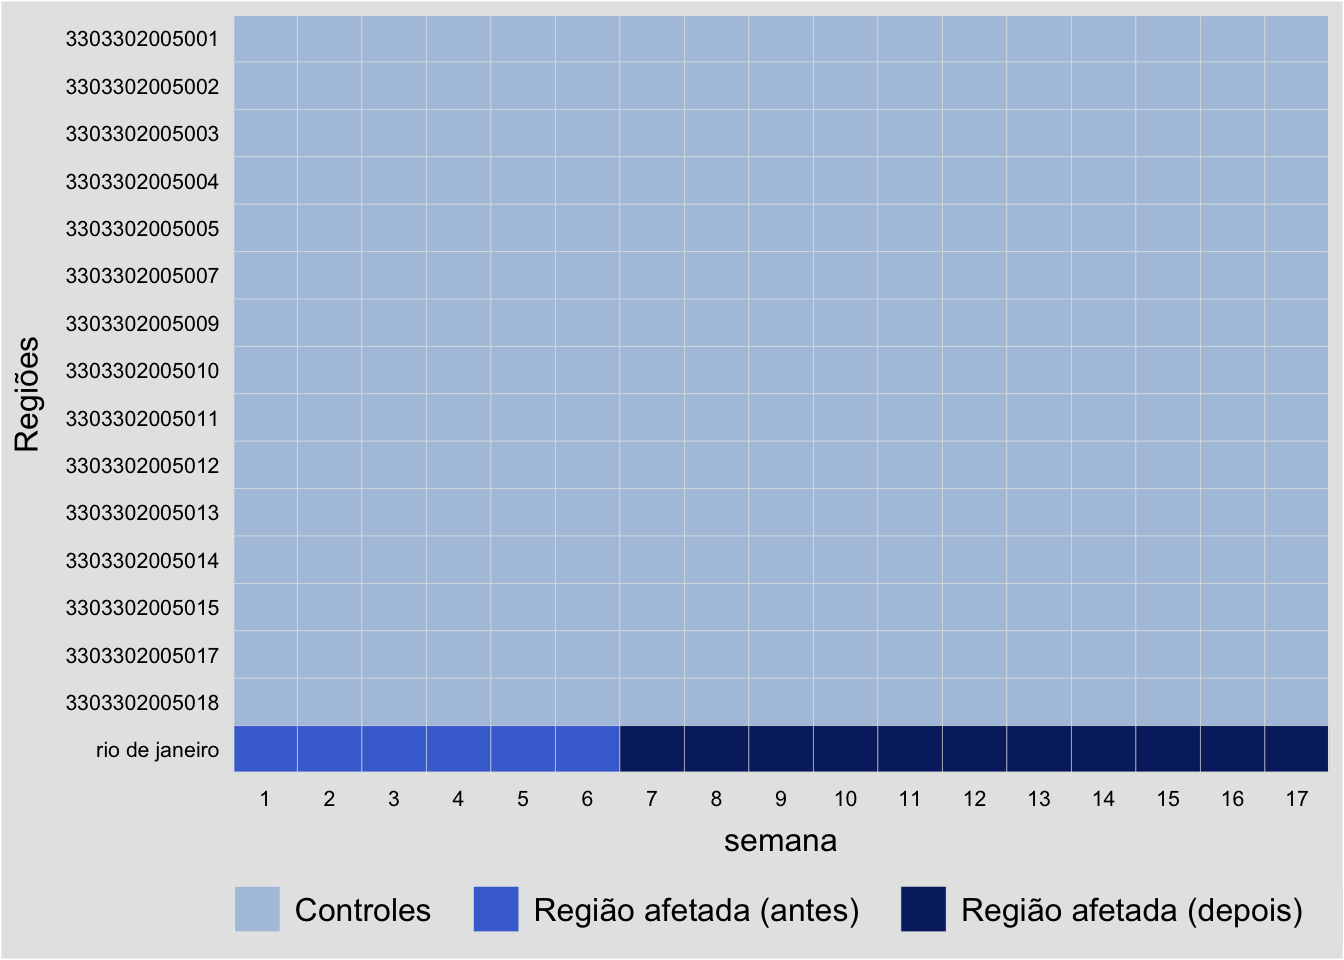
\includegraphics{dissertacao-demo_files/figure-latex/tabelaSynth0-1} 

}

\caption{Dados em painel.}\label{fig:tabelaSynth0}
\end{figure}

Conforme é possível observar na figura \ref{fig:tabelaSynth0}, trata-se de um painel balanceado. O evento ocorre a partir da semana 7. As regiões representadas por números são as áreas de ponderação.

Na figura \ref{fig:graficoSynth1} é possível observar o comportamento da receita ao longo do período analisado. Nesta figura, o município do Rio de Janeiro é representado pela linha preta e as demais áreas de ponderação são representadas pelas linhas claras em azul. Como podemos observar, o comportamento do município do RJ é semelhante ao de seus controles, antes do evento (área cinza claro). Após o evento (área cinza escuro) percebe-se uma forte elevação de receita no RJ, que não é observado nos controles. A linha azul tracejada representa o controle sintético (contrafactual), gerado pelo modelo.

\begin{figure}

{\centering 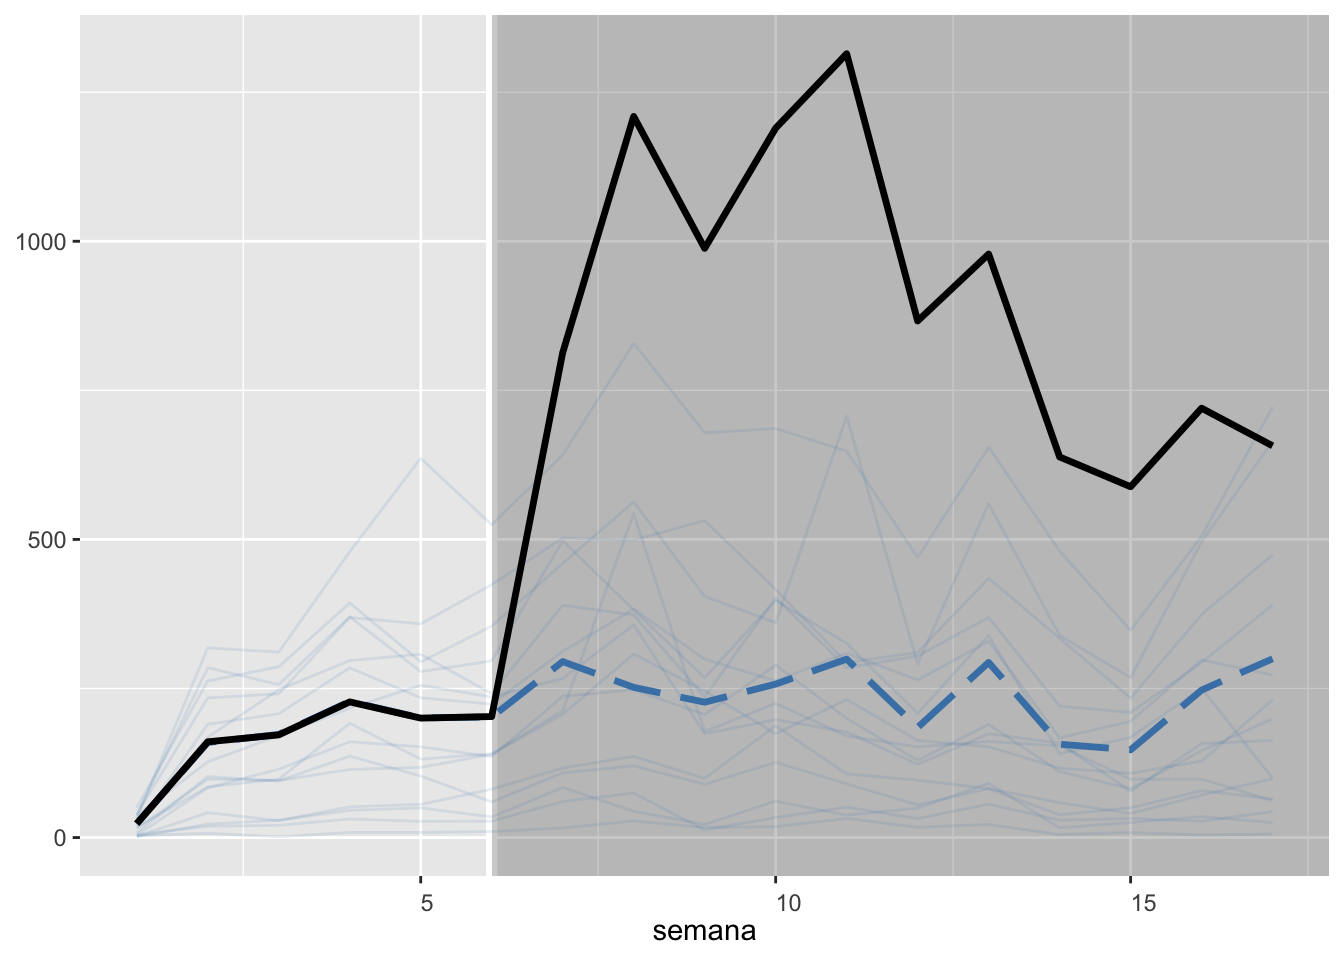
\includegraphics{dissertacao-demo_files/figure-latex/graficoSynth1-1} 

}

\caption{controle sintético da receita com água mineral.}\label{fig:graficoSynth1}
\end{figure}

Na Tabela \ref{tab:tabelaSynth} estão representados os impactos estimados do evento em cada semana. A coluna ATT ( \emph{average treatment effect on treated} ) representa esse impacto. A coluna ``n.Treated'' representa a presença ou ausência do evento. Na semana 7, inicio do evento, ocorre um aumento de R\$ 518,00 na receita para cada mil habitantes e esse valor alcança R\$ 1.015,18 na semana 11.

\begin{table}

\caption{\label{tab:tabelaSynth}Impacto estimado em cada semana.}
\centering
\begin{tabular}[t]{rrrrrrr}
\toprule
semana & ATT & S.E. & CI.lower & CI.upper & p.value & n.Treated\\
\midrule
\addlinespace[2em]
\multicolumn{7}{l}{\textbf{pré evento}}\\
\hspace{1em}\cellcolor{gray!6}{1} & \cellcolor{gray!6}{-0.172} & \cellcolor{gray!6}{5.908} & \cellcolor{gray!6}{-16.217} & \cellcolor{gray!6}{9.506} & \cellcolor{gray!6}{0.570} & \cellcolor{gray!6}{0}\\
\hspace{1em}2 & 1.190 & 17.402 & -33.498 & 39.568 & 0.844 & 0\\
\hspace{1em}\cellcolor{gray!6}{3} & \cellcolor{gray!6}{-0.769} & \cellcolor{gray!6}{16.467} & \cellcolor{gray!6}{-26.205} & \cellcolor{gray!6}{43.046} & \cellcolor{gray!6}{0.802} & \cellcolor{gray!6}{0}\\
\hspace{1em}4 & -0.632 & 14.184 & -34.066 & 25.554 & 0.684 & 0\\
\hspace{1em}\cellcolor{gray!6}{5} & \cellcolor{gray!6}{-0.279} & \cellcolor{gray!6}{10.962} & \cellcolor{gray!6}{-21.441} & \cellcolor{gray!6}{22.336} & \cellcolor{gray!6}{0.890} & \cellcolor{gray!6}{0}\\
\hspace{1em}6 & 0.663 & 13.984 & -31.806 & 29.646 & 0.928 & 0\\
\addlinespace[2em]
\multicolumn{7}{l}{\textbf{pós evento}}\\
\hspace{1em}\cellcolor{gray!6}{7} & \cellcolor{gray!6}{518.011} & \cellcolor{gray!6}{75.860} & \cellcolor{gray!6}{377.022} & \cellcolor{gray!6}{622.825} & \cellcolor{gray!6}{0.006} & \cellcolor{gray!6}{1}\\
\hspace{1em}8 & 957.443 & 252.952 & 409.072 & 1341.321 & 0.002 & 1\\
\hspace{1em}\cellcolor{gray!6}{9} & \cellcolor{gray!6}{761.126} & \cellcolor{gray!6}{151.744} & \cellcolor{gray!6}{573.097} & \cellcolor{gray!6}{994.369} & \cellcolor{gray!6}{0.010} & \cellcolor{gray!6}{1}\\
\hspace{1em}10 & 932.349 & 190.213 & 750.074 & 1142.563 & 0.010 & 1\\
\hspace{1em}\cellcolor{gray!6}{11} & \cellcolor{gray!6}{1015.189} & \cellcolor{gray!6}{402.975} & \cellcolor{gray!6}{399.266} & \cellcolor{gray!6}{1843.734} & \cellcolor{gray!6}{0.006} & \cellcolor{gray!6}{1}\\
\hspace{1em}12 & 681.732 & 149.946 & 517.140 & 897.731 & 0.010 & 1\\
\hspace{1em}\cellcolor{gray!6}{13} & \cellcolor{gray!6}{684.822} & \cellcolor{gray!6}{222.379} & \cellcolor{gray!6}{419.485} & \cellcolor{gray!6}{1063.863} & \cellcolor{gray!6}{0.006} & \cellcolor{gray!6}{1}\\
14 & 481.755 & 125.051 & 286.373 & 720.943 & 0.004 & 1\\
\cellcolor{gray!6}{15} & \cellcolor{gray!6}{441.294} & \cellcolor{gray!6}{128.765} & \cellcolor{gray!6}{289.313} & \cellcolor{gray!6}{667.232} & \cellcolor{gray!6}{0.008} & \cellcolor{gray!6}{1}\\
16 & 472.756 & 194.524 & 210.218 & 827.202 & 0.010 & 1\\
\cellcolor{gray!6}{17} & \cellcolor{gray!6}{357.044} & \cellcolor{gray!6}{423.658} & \cellcolor{gray!6}{-256.200} & \cellcolor{gray!6}{1221.183} & \cellcolor{gray!6}{0.182} & \cellcolor{gray!6}{1}\\
\bottomrule
\end{tabular}
\end{table}

Os mesmos dados da Tabela \ref{tab:tabelaSynth} podem ser visualizados na Figura \ref{fig:graficoSynth2}. No período pré-evento, o efeito é nulo. Após o evento, observa-se um forte deslocamento para cima na estimativa do efeito e somente na ultima semanda o efeito perde significância estatistica.

\begin{figure}

{\centering 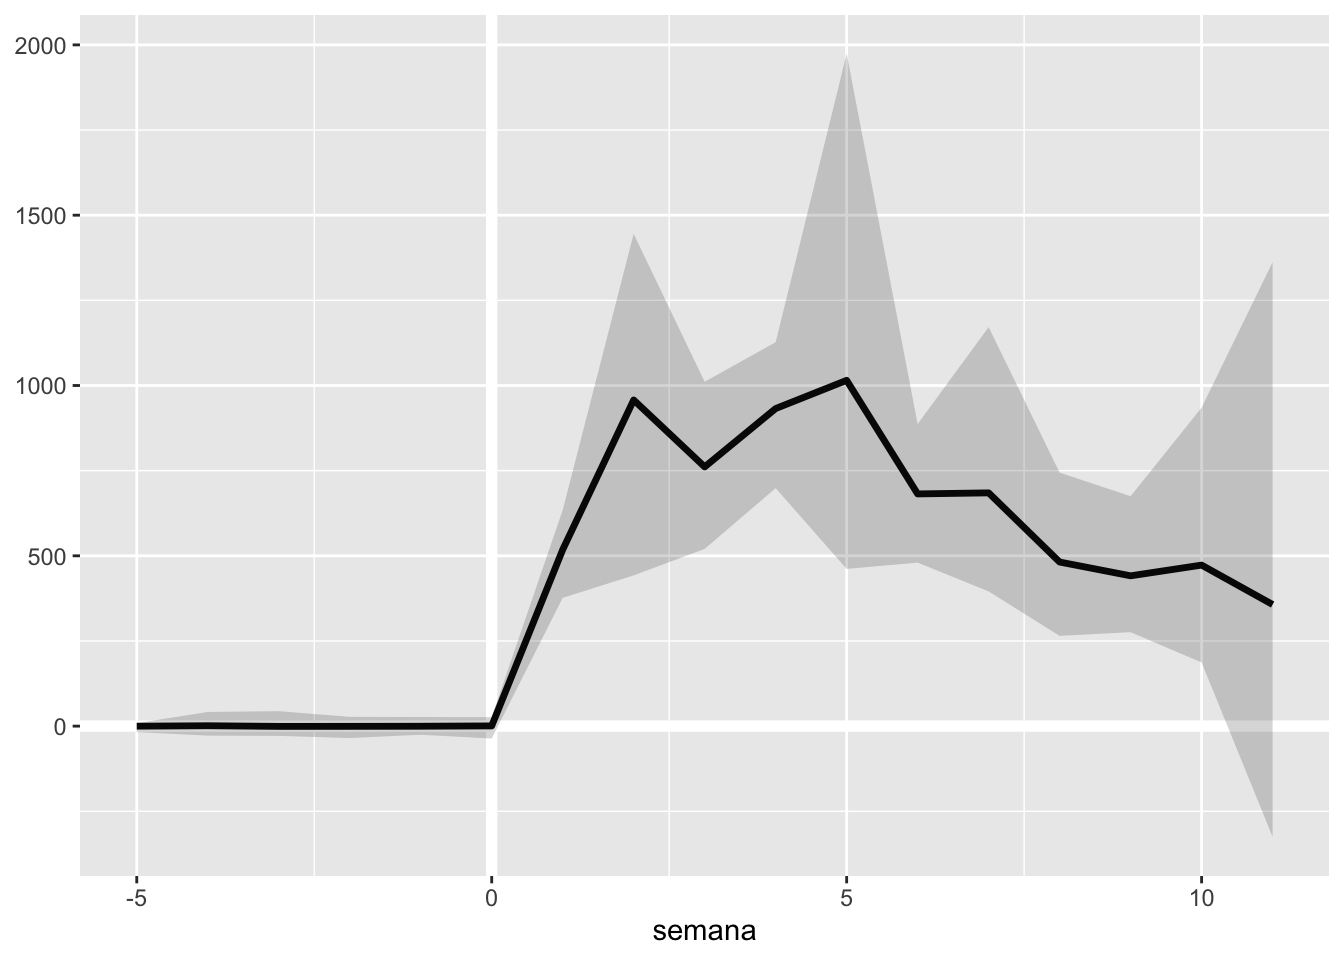
\includegraphics{dissertacao-demo_files/figure-latex/graficoSynth2-1} 

}

\caption{controle sintético e estimativa de impacto.}\label{fig:graficoSynth2}
\end{figure}

\hypertarget{conclusuxe3o}{%
\chapter{Conclusão}\label{conclusuxe3o}}

O presente estudo procurou estimar a disposição a pagar via preferencias reveladas utilizando como arcabouço o impacto da crise hídrica da estação de tratamento Guandu nos gastos com água mineral do município do Rio de Janeiro. O impacto foi medido pelo aumento das receitas decorrentes da venda no varejo de água mineral. Sendo que, a receita é uma combinação de duas variáveis: preço e quantidade. Como cada uma destas variáveis apresenta caracteristicas econômicas próprias, realizou-se uma análise para cada variável.

Sob a ótica da quantidade, o evento gerou um impacto de aumentar em 292\% a demanda. Enquanto que em relação ao preço, o evento gerou um aumento de 26,5\% no mesmo.

Avaliar o aumento da receita de vendas de água mineral pode ser utilizado como uma \emph{proxy} da WTP por água potável. Quando a WTP é avaliada a partir do gasto mensal do domicílio, este estudo encontrou um valor de U\$ 7,89, ou seja, este foi o valor médio do gasto domiciliar no mês de fevereiro de 2020. Valor próximo ao encontrados por outros autores (\citet{wtpmalawi} e \citet{wtpespiritosanto}).

Além disso, o impacto total do evento, quando medido através da receita total com água mineral no período de janeiro a março foi estimado em R\$ 79 milhões. Tal impacto foi medido apenas na cidade do Rio de Janeiro, sendo que o referido problema ocorreu em diversos municípios da Região Metropolitana do estado do Rio de Janeiro.

Contudo, devemos ressaltar que a aquisição de água mineral não é a única forma de contornar a questão do fornecimento de água encanada de baixa qualidade. Diversos estudos (\citet{migueldoria}, \citet{franzfoltz}, \citet{wtpespiritosanto}, \citet{serret}) apontam que outras alternativas comumente adotadas incluem a aquisição de filtros ou a fervura da água, os quais apresentam seus próprios custos. Tais custos não foram considerados no presente estudo.

Para exemplificar o tamanho do mercado de água mineral, em setembro de 2020, o fundador da empresa Nongfu, gigante chinesa de produção de água engarrafada, se tornou o homem mais rico da China e o décimo sétimo do mundo. A empresa chegou a captar U\$ 1 bilhão durante a IPO na bolsa de valores de Hong Kong.

Em relação à elasticidade preço da demanda observado em nosso estudo, este ficou em 2,49, demonstrando uma alta elasticidade. Neste ponto cabe citar estudo realizado no Espírito Santo \citep{wtpespiritosanto} no qual os autores observaram que apenas 4\% da população estudada utilizava água mineral. Ou seja, em regra, a água mineral é um bem não essencial.

Em estudo realizado na espanha \citep{martasuarez}, onde os autores relatam ser o nono maior país do mundo em consumo de água mineral, foi observado que 32,2\% da população consumia água mineral regularmente e a média de consumo foi de 4,3 litros por habitante por semana. Ou seja, apesar da água ser um bem essencial, a água mineral não apresenta essa mesma caracteristica.

Com relação às externalidades, o consumo de água mineral gera uma maior produção de residuos não biodegradáveis decorrentes das garrafas plásticas, os quais trazem forte impacto para o meio ambiente. Ainda temos o maior consumo energético necessário para a produção de água mineral quando comparado a produção de água encanada, podendo chegar a um consumo 2000 vezes maior de energia\citep{martasuarez}.

  \bibliography{book.bib,packages.bib}

\end{document}
